
\section{Exercises}

\subsection{Paired data}

{\dph{
\eoce{Is there strong evidence that the continental U.S. is warming? We might take a simple approach to this problem and compare how temperatures have changed from 1968 to 2008. The daily high temperature reading on January 1 was collected for 1968 and 2008 for 51 randomly selected locations in the continental US. Then the difference between the two readings (temperature in 2008 - temperature in 1968) was calculated for each of the 51 different locations. The average of these 51 values was 1.1 degrees with a standard deviation of 4.9 degrees. We are interested in finding out if these data provide convincing evidence of temperature warming in the continental US.
\begin{enumerate}[(a)]
\setlength{\itemsep}{0mm}
\item Are the two data sets of 51 observations dependent or independent of each other? Based on this, what type of analysis should be conducted to test if these data provide convincing evidence of temperature warming in the continental US.
\item Are the assumptions and conditions for inference satisfied?
\item Write the hypotheses in symbols and in words.
\item Calculate the test statistic and find the p-value.
\item What do you conclude? Interpret your conclusion in context.
\item What type of error might we have committed? Explain in context what the error means.
\item Based on the result of this hypothesis test, would you expect a confidence interval for the average difference between the temperature measurements from 1968 and 2008 to include 0? Explain your reasoning.
\end{enumerate}
}
{
\begin{enumerate}[(a)]
\item The observations in the two data sets are dependent since they are recorded at the same location; therefore, a hypothesis test for paired data should be used for this analysis.
\item 
\begin{enumerate}[1.]
\item Independence Assumption: 
\begin{itemize}
\item Random Sampling Condition: We are told that locations are sampled randomly.
\item 10\% Condition: 51 $<$ 10\% of all locations in the continental US.
\end{itemize}
Since we have a random sample and the 10\% condition is satisfied, we can assume that the temperature in one location is independent of another.
\item Nearly Normal Condition: As long as the distributions of the daily high temperatures on January 1 on 1968 and 2008 are not extremely skewed, $n > 50$ should be large enough to assume that the both sample means are normally distributed.
\item Dependent Groups: The two samples are dependent on each other.
\end{enumerate}
\item $H_0: \mu_{diff} = 0$ (There is no difference in average daily high temperature between January 1, 1968 and January 1, 2008) \\
$H_0: \mu_{diff} > 0$ (Average daily high temperature in January 1, 1968 was lower than average daily high temperature in January, 2008.)
\item The test statistic and the p-value can be calculated as follows:
\[ Z = \frac{\bar{x}_{diff} - \mu_{diff}}{ \frac{s_{diff}}{\sqrt{n}} } = \frac{1.1 - 0}{\frac{4.9}{\sqrt{51}}} = \frac{1.1}{0.6861} = 1.60 \]
\[ p-value = P(Z > 1.60) = 1 - 0.9452 = 0.0548 \]
\item Since p-value $> \alpha$ (since not given use 0.05), fail to reject $H_0$. The data do not provide convincing evidence of temperature warming in the continental US. However it should be noted that the p-value is very close to 0.05.
\item Type II, since we failed to reject $H_0$. If we made such an error and concluded that there isn't convincing evidence for temperature warming in the continental US, but in reality average temperature on January 1, 2008 is significantly higher than average temperature on January 1, 1968.
\item Since we failed to reject $H_0$ which claimed the average difference is equal to 0, we would expect a confidence interval to include this value.
\end{enumerate}
}\label{temperatureWarming}
}}

%

{
\eoce{In Exercise~\eoceref{temperatureWarming} we considered the differences between the temperature readings in January 1 of 1968 and 2008 at 51 locations in the continental US.
\begin{enumerate}[(a)]
\setlength{\itemsep}{0mm}
\item Calculate a 90\% confidence interval for the average difference between the temperature measurements from 1968 and 2008.
\item Interpret this interval in context.
\item Does this interval agree with the conclusion of the hypothesis test from Exercise~\eoceref{temperatureWarming}? Explain.
\end{enumerate}
}
{
\begin{enumerate}[(a)]
\item A 90\% confidence interval can be calculated as follows:
\begin{align*}
\bar{x}_{diff} \pm z^* \frac{s_{diff}}{\sqrt{n}} &= 1.1 \pm 1.645 \frac{4.9}{\sqrt{51}} \\
&= 1.1 \pm 1.645 * 0.6861 \\
&= 1.1 \pm 1.13 \\
&= (-0.03, 2.23)
\end{align*}
\item We are 90\% confident that the average daily high in January 1, 2008 in the continental US was 0.13 degrees lower to 2.13 degrees higher than the average daily high in January 1, 1968.
\item Yes, we failed to reject $H_0$ which claimed the average difference is equal to 0, and the interval includes this value.
\end{enumerate}
}
}

%

\subsection{Difference of two means}

% Point estimates and standard errors for differences of means

% Confidence interval for the difference

% Hypothesis test based on a difference in means

\eoce{In 1964 the Surgeon General released their first report linking smoking to various health issues, including cancer. Research done by Sterling Cooper, a prestigious ad agency in New York City, showed that before the report was released, in a random sample of 80 smokers, the average number of cigarettes smoked per day was 13.5 with a standard deviation of 3.2. A year after the report was released, in a random sample of 85 smokers, the average number of cigarettes smoked per day was 12.6 with a standard deviation of 2.9. Is there evidence to suggest that the average number of cigarettes smoked per day has decreased after the Surgeon General's report?

\begin{center}
\begin{tabular}{c|cc}
 & Before & After \\
\hline
n & 80 & 85 \\
$\bar{x}$ & 13.5 & 12.6 \\
s & 3.2 & 2.9
\end{tabular}
\end{center}

\begin{enumerate}[(a)]
\setlength{\itemsep}{0mm}
\item Write the hypotheses in symbols and in words.
\item Are the assumptions and conditions for inference satisfied?
\item Calculate the test statistic and find the p-value.
\item What do you conclude? Interpret your conclusion in context.
\item Does this imply that the Surgeon General's report was the cause of this decrease? Explain.
\item What type of error might we have committed? Explain.
\end{enumerate}
}
{
\begin{enumerate}[(a)]
\item Let $\mu_1$ denote population mean Before, and $\mu_2$ denote population mean After.

$H_0: \mu_1 = \mu_2 \rightarrow \mu_1 - \mu_2 = 0$ (The population mean of number of cigarettes smoked per day did not change after the Surgeon General's report) \\
$H_A: \mu_1 > \mu_2 \rightarrow \mu_1 - \mu_2 > 0$ (The population mean of number of cigarettes smoked per day has decreased after the Surgeon General's report)

\item
\begin{enumerate}[1.]
\item Independence Assumption: 
\begin{itemize}
\item Random Sampling Condition: We are told that the sample is random.
\item 10\% Condition: 80 and 82 $<$ 10\% of smokers in the 1960s.
\end{itemize}
Since we have a random sample and the 10\% condition is satisfied, we can assume that the number of cigarettes smoked by the subjects are independent of each other.
\item Nearly Normal Condition: As long as the distributions of number of cigarettes smoked per day before and after the report was released are not extremely skewed, $n > 50$ should be large enough to assume that the both sample means are normally distributed.
\item Independent Groups: The two samples are independent of each other.
\end{enumerate}

\item The test statistic and the p-value can be calculated as follows:
\[ Z = \frac{(\bar{x}_1 - \bar{x_2}) - (\mu_1 - \mu_2)}{\sqrt{ \frac{s_1^2}{n_1} + \frac{s_2}{n_2} }} = \frac{(13.5 - 12.6) - 0}{ \sqrt{\frac{3.2^2}{80} + \frac{2.9^2}{85}} } = 1.89 \]
\[ p-value = P(z > 1.89) = 1 - 0.9706 = 0.0294 \]

\item Since p-value $< \alpha$ (since not given use 0.05), reject $H_0$. There is sufficient evidence to suggest that the number of cigarettes smoked per day has decreased after the Surgeon General's report.

\item No, the result of the hypothesis test does not imply causation.

\item Type I, since we rejected $H_0$.

\end{enumerate}
}\label{SterlingCooper}

%

\eoce{Based on the data given in Exercise~\eoceref{SterlingCooper}, construct a 90\% confidence interval for the difference between the average number of cigarettes smoked per day before and after the Surgeon General's report was released. Interpret this interval in context. Also comment on if the confidence interval agrees with the conclusion of the hypothesis test from Exercise~\eoceref{SterlingCooper}. 
}
{
A 90\% confidence interval can be calculated as follows:
\begin{align*}
(\bar{x}_1 - \bar{x}_2) \pm z^* \sqrt{ \frac{s_1^2}{n_1} + \frac{s_2^2}{n_2} } &= (13.5 - 12.6) \pm 1.645 * \sqrt{\frac{3.2^2}{80} + \frac{2.9^2}{85}} \\
&= 0.9 \pm 1.645 * 0.4764 \\
&= 0.9 \pm 0.78 \\
&= (0.12, 1.68)
\end{align*}

We are 90\% confident that the average number of cigarettes smoked per day before the report was released is 0.12 to 1.68 higher than the average number of cigarettes smoked after the report was released.

Yes, in Exercise~\eoceref{SterlingCooper} we rejected $H_0$ which claims that the two population means are equal to each other, and the confidence interval does not include 0.
}

%

{\dph{
\eoce{In 1990 and 2004 the National Assessment of Educational Progress program tested 17 year old students in mathematics. In each of these two years, 1,000 students were randomly sampled from US schools. The average score changed from 305 in 1990 to 307 in 2004. The standard deviation for the 1990 data was 34, and for the 2004 data was 27. We are interested in finding out if there has been a change in the average math scores between 1990 and 2004.
\begin{enumerate}[(a)]
\setlength{\itemsep}{0mm}
\item Write the hypotheses in symbols and in words.
\item Are the assumptions and conditions for inference satisfied?
\item Calculate the test statistic and find the p-value.
\item What do you conclude? Interpret your conclusion in context.
\item What type of error might we have committed? Explain.
\end{enumerate}
}
{
\begin{enumerate}[(a)]
\item Let $\mu_1$ denote average score in 1990, and $\mu_2$ denote average score in 2004. \\
$H_0: \mu_1 = \mu_2 \rightarrow \mu_1 - \mu_2 = 0$ (Average math score in 1990 is equal to average math score in 2004) \\
$H_A: \mu_1 > \mu_2 \rightarrow \mu_1 - \mu_2 > 0$ (Average math score in 1990 is different than average math score in 2004)
\item
\begin{enumerate}[1.]
\item Independence Assumption: 
\begin{itemize}
\item Random Sampling Condition: We are told that both samples are random
\item 10\% Condition: 1000 $<$ 10\% of students in 1990 an 2004.
\end{itemize}
Since we have a random sample and the 10\% condition is satisfied, we can assume that the how well one student in the sample scores on the exam is independent of another.
\item Nearly Normal Condition: As long as the distribution of scores in 1990 and 2004 are not extremely skewed, such a large sample size should be enough to assume that the both sample means are normally distributed.
\item Independent Groups: Both are random samples from two different years, so we have no reason to think the samples would not be independent of each other.
\end{enumerate}
\item The test statistic and the p-value can be calculated as follows:
\[ Z = \frac{(\bar{x}_1 - \bar{x_2}) - (\mu_1 - \mu_2)}{\sqrt{ \frac{s_1^2}{n_1} + \frac{s_2}{n_2} }} = \frac{(305 - 307) - 0}{ \sqrt{\frac{34^2}{1000} + \frac{27^2}{1000}} } = \frac{-2}{1.3730} = -1.46 \]
\[ p-value = P(|z| > -1.46) = 2 * 0.0721 = 0.1442 \]
\item Since p-value $> \alpha$ (since not given use 0.05), fail to reject $H_0$. The data do not provide convincing evidence to suggest that the average score has changed between 1990 and 2004.
\item Type II, since we failed to reject $H_0$.
\end{enumerate}
}\label{mathScore}
}}

%

{
\eoce{Based on the data given in Exercise~\eoceref{mathScore}, construct a 90\% confidence interval for the difference between the average scores in 1990 and 2004. Interpret this interval in context. Also comment on if the confidence interval agrees with the conclusion of the hypothesis test from Exercise~\eoceref{mathScore}. 
}
{
A 90\% confidence interval can be calculated as follows:
\begin{align*}
(\bar{x}_1 - \bar{x}_2) \pm z^* \sqrt{ \frac{s_1^2}{n_1} + \frac{s_2^2}{n_2} } &= (305 - 307) \pm 1.645 *  \sqrt{\frac{34^2}{1000} + \frac{27^2}{1000}} \\
&= -2 \pm 1.645 * 1.3730 \\
&= -2 \pm 2.26 \\
&= (-4.26, 0.26)
\end{align*}
We are 90\% confident that the average score in 1990 was 4.26 points lower to 0.26 point higher than the average score in 2004. This agrees with the conclusion of the hypothesis test from Exercise~\eoceref{mathScore}; we failed to reject $H_0$ which claims that the two population means are equal, and the confidence interval includes 0.
}
}

%

\eoce{An article published in the International Journal of Obesity \citep{Romero:2008} examined the accuracy of BMI in diagnosing obesity. Data from 13,601 subjects aged 20-79.9 from the Third National Health and Nutrition Examination Survey were studied. Two of the variables of interest were body fat percentage (BF) and lean mass. Below is an excerpt of some of results of this study. Note that BMI, BF and lean mass are given as \textit{mean $\pm$ standard error}. Assume that all assumptions and conditions for inference are satisfied.
\begin{center}
\begin{tabular}{l c c c}
\hline
Gender	& n		& BF (\%)			& Lean mass (kg)	\\
\hline
Men		& 6580	& 23.9 $\pm$ 0.07	& 61.8 $\pm$ 0.12 \\
Women	& 7021	& 35.0 $\pm$ 0.09	& 44.0 $\pm$ 0.08 \\
\hline
\end{tabular}
\end{center}

\begin{enumerate}[(a)]
\setlength{\itemsep}{0mm}
\item One definition of obesity in women is greater than 35\% body fat and in men greater than 25\%. The cutoff for women is higher since women store extra fat in their bodies to be used during childbearing. This implies that women on average should have a higher body fat percentage than men. Test this hypothesis using $\alpha = 0.01$.
\item Lean mass and fat mass are what makes up a person's total weight. In part (a) we showed that women on average have higher body fat percentage. The data also show that women have lower mean mass. Is the only reason for this higher body fat percentage, or can you think of other reasons why women on average have lower lean mass?
\end{enumerate}
}
{
\begin{enumerate}[(a)]
\item Let $\mu_1$ denote population mean for men, and $\mu_2$ denote population mean for women.

$H_0: \mu_1 = \mu_2$ (There is no difference between the average BF\% of men and women.) \\
$H_A: \mu_1 < \mu_2$ (Average BF\% of women is higher than average BF\% for men.)

Before we can do the hypothesis test we must first calculate the standard deviations of the two samples. Remember, $SE = \frac{s}{\sqrt{n}}$. \\

\begin{minipage}[c]{0.5\textwidth}
\begin{center}
Men: 
\begin{align*}
0.07 &= \frac{s}{\sqrt{6580}} \\
s &= 0.07 * \sqrt{6580} \\
&= 5.68
\end{align*}
\end{center}
\end{minipage}
\begin{minipage}[c]{0.5\textwidth}
\begin{center}
Women: 
\begin{align*}
0.09 &= \frac{s}{\sqrt{7021}} \\
s &= 0.09 * \sqrt{7021} \\
&= 7.54
\end{align*}
\end{center}
\end{minipage}

The test statistic and the p-value can be calculated as follows:
\[ Z = \frac{(\bar{x}_1 - \bar{x_2}) - (\mu_1 - \mu_2)}{\sqrt{ \frac{s_1^2}{n_1} + \frac{s_2}{n_2} }} = \frac{(23.9 - 35.0) - 0}{ \sqrt{\frac{5.68 ^2}{6580} + \frac{7.54 ^2}{7021}} } = -97.35 \]
\[ p-value = P(|z| > -97.35) \approx 0 \]

Since p-value $< \alpha$, reject $H_0$. There is sufficient evidence to suggest that average body fat percentage for women is higher.

\item Women on average tend to weigh less than men. Therefore their lean mass is bound to be lower than that of men.

\end{enumerate}

}

%

% Examining the standard error formula

%%%

\subsection{Single population proportion}

%%%

{
\eoce{Suppose that 8\% of college students are vegetarians. Based on this information, determine if the following statements are true or false. Explain your reasoning.
\begin{enumerate}[(a)]
\setlength{\itemsep}{0mm}
\item The distribution of the sample proportions of vegetarians in random samples of size 60 is nearly normal since $n \ge 50$. 
\item The distribution of the sample proportions of vegetarian college students in random samples of size 50 is right skewed.
\item A random sample of 125 college students where 12\% are vegetarians would be considered unusual. 
\item A random sample of 250 college students where 12\% are vegetarians would be considered unusual.
\item Increasing the sample size from 125 to 250 would cut in half the standard error of the sample proportion.
\end{enumerate}
}
{
\begin{enumerate}[(a)]
\item FALSE. For the distribution of $\hat{p}$ to be nearly normal, we need to have at least 10 successes and 10 failures in our sample. Unlike with means, with proportions for the distribution of the sample statistics ($\hat{p}$) to be nearly normal, we need to have at least 10 successes and 10 failures in our sample. We do not use $n \ge 50$ as a condition to check for the normality of the distribution of $\hat{p}$.
\item TRUE. The success-failure condition is not satisfied
\[ n\hat{p} = 50 * 0.08 = 4~and~ n\hat{q} = 50 * 0.92 = 46, \]
therefore we know that the distribution of $\hat{p}$ is not nearly normal. In most samples we would expect $\hat{p}$ to be close to 0.08, the true population proportion. While $\hat{p}$ can be as high as 1 (though we would expect this to happen very rarely), it can only go as low as 0. Therefore the distribution would probably take on a right-skewed shape. Plotting the sampling distribution would confirm this suspicion.
\item FALSE. Standard error of $\hat{p}$ in samples with $n = 125$ can be calculated as:
\[SE_{\hat{p}} = \sqrt{ \frac{pq}{n} } = \sqrt{\frac{0.08 * 0.92}{125}} = 0.0243 \]
A $\hat{p}$ of 0.12 is only $\frac{0.12 - 0.08}{0.0243} = 1.65$ standard errors away from the mean, which would not be considered unusual.
\item TRUE. Standard error of $\hat{p}$ in samples with $n = 125$ can be calculated as:
\[SE_{\hat{p}} = \sqrt{ \frac{pq}{n} } = \sqrt{\frac{0.08 * 0.92}{250}} = 0.0172 \]
A $\hat{p}$ of 0.12 is only $\frac{0.12 - 0.08}{0.0172} = 2.32$ standard errors away from the mean, which might be considered unusual.
\item FALSE. Since $n$ appears under the square root sign in the formula for the standard error, increasing the sample size from 125 to 250 would decrease the standard error of the sample proportion only by a factor of $\sqrt{2}$.
\end{enumerate}
}
}

%

{
\eoce{Given that 90\% of all orange tabby kittens born are males, which of the following statements are true? Based on this information, determine if the following statements are true or false. Explain your reasoning. 
\begin{enumerate}[(a)]
\setlength{\itemsep}{0mm}
\item The distribution of sample proportions of samples of size 30 is left skewed.
\item Doubling the sample size will reduce the standard error of the sample proportion by $\frac{1}{2}$.
\item The distribution of sample proportions of samples of size 140 is approximately normal.
\item Doubling the sample size will reduce the standard error of the sample proportion by $\frac{1}{\sqrt{2}}$.
\item The distribution of sample proportions of samples of size 70 is approximately normal.
\end{enumerate}
}
{
\begin{enumerate}[(a)]
\item TRUE. The success-failure condition is not satisfied
\[ n\hat{p} = 30 * 0.90 = 27~and~ n\hat{q} = 30 * 0.10 = 3, \]
therefore we know that the distribution of $\hat{p}$ is not nearly normal. In most samples we would expect $\hat{p}$ to be close to 0.90, the true population proportion. While $\hat{p}$ can be as low as 0 (thought we would expect this to happen very rarely), it can only go as high as 1. Therefore the distribution would probably take on a left-skewed shape. Plotting the sampling distribution would confirm this suspicion.
\item FALSE.  Since $n$ appears under the square root sign in the formula for the standard error, doubling the sample size would decrease the standard error of the sample proportion only by a factor of $\sqrt{2}$.
\item TRUE. The success-failure condition is satisfied
\[ n\hat{p} = 140 * 0.90 = 126 ~and~ n\hat{q} = 140 * 0.10 = 14, \]
therefore the distribution of $\hat{p}$ is nearly normal.
\item TRUE. 
\[ SE_{old} =  \sqrt{\frac{\hat{p}\hat{q}}{n}} ~\hspace{1cm}~ SE_{new} = \sqrt{\frac{\hat{p}\hat{q}}{2n}} = \frac{1}{\sqrt{2}} \sqrt{\frac{\hat{p}\hat{q}}{n}} = \frac{1}{\sqrt{2}}ME_{old}\]
\item FALSE. The success-failure condition is not satisfied
\[ n\hat{p} = 70 * 0.90 = 63 ~and~ n\hat{q} = 70 * 0.10 = 7, \]
therefore the distribution of $\hat{p}$ is not nearly normal.
\end{enumerate}
}
}

%

{
\eoce{Suppose that the proportion of the adult population who jog is 0.15. Based on this information, determine if the following statements are true or false. Explain your reasoning. 
\begin{enumerate}[(a)]
\setlength{\itemsep}{0mm}
\item The distribution of the proportions of joggers in random samples of size 40 is right skewed.
\item The distribution of the proportions of joggers in random samples of size 65 is nearly normal since $n \ge 50$. 
\item A random sample of 150 where 20\% are joggers would be considered unusual. 
\item A random sample of 300 where 20\% are joggers would be considered unusual.
\item Increasing the sample size from 150 to 300 would cut in half the standard error of the sample proportion.
\end{enumerate}
}
{
\begin{enumerate}[(a)]
\item TRUE. The success-failure condition is not satisfied
\[ n\hat{p} = 40 * 0.15 = 6~and~ n\hat{q} = 40 * 0.85 = 34, \]
therefore we know that the distribution of $\hat{p}$ is not nearly normal. In most samples we would expect $\hat{p}$ to be close to 0.15, the true population proportion. While $\hat{p}$ can be as high as 1 (thought we would expect this to happen very rarely), it can only go as low as 0. Therefore the distribution would take on a right skewed shape.
\item FALSE. For the distribution of $\hat{p}$ to be nearly normal, we need to have at least 10 successes and 10 failures in our sample. Unlike with means, with proportions for the distribution of the sample statistics ($\hat{p}$) to be nearly normal, we need to have at least 10 successes and 10 failures in our sample. We do not use $n \ge 50$ as a condition to check for the normality of the distribution of $\hat{p}$.
\item FALSE. Standard error of $\hat{p}$ in samples with $n = 150$ can be calculated as:
\[SE_{\hat{p}} = \sqrt{ \frac{pq}{n} } = \sqrt{\frac{0.15 * 0.85}{150}} = 0.0292 \]
A $\hat{p}$ of 0.12 is only $\frac{0.22 - 0.15}{0.0357} = 1.71$ standard errors away from the mean, which would not be considered unusual.
\item TRUE. Standard error of $\hat{p}$ in samples with $n = 300$ can be calculated as:
\[SE_{\hat{p}} = \sqrt{ \frac{pq}{n} } = \sqrt{\frac{0.15 * 0.85}{300}} = 0.0206 \]
A $\hat{p}$ of 0.12 is only $\frac{0.22 - 0.15}{0.0206} = 2.43$ standard errors away from the mean, which might be considered unusual.
\item FALSE. Since $n$ appears under the square root sign in the formula for the standard error, increasing the sample size from 150 to 300 would decrease the standard error of the sample proportion only by a factor of $\sqrt{2}$.
\end{enumerate}
}
}

% Confidence intervals for a proportion

{
\eoce{In a poll conducted by Survey USA on July 12, 2010 70\% of the 119 respondents between the ages of 18 and 34 said they will vote in the 2010 general election for Prop 19 which would change California law to legalize marijuana and allow it to be regulated and taxed. At a 95\% confidence level this sample has an 8\% margin of error. Based on this information, determine if the following statements are true or false. Explain your reasoning.
\begin{enumerate}[(a)]
\setlength{\itemsep}{0mm}
\item We are 95\% confident that between 62\% and 78\% of the California voters in this sample support support Prop 19.
\item We are 95\% confident that between 62\% and 78\% of all California voters between the ages of 18 and 34 support Prop 19.
\item If we considered many random samples of 119 California voters between the ages of 18 and 34 calculated the sample proportions of those who support Prop 19, 95\% of them will be between 62\% and 78\%.
\item In order to decrease the margin of error to 4\% we would need to quadruple (multiply by 4) the sample size.
\item Based on this confidence interval there is sufficient evidence to suggest that majority of California voters between the ages of 18 and 34 support Prop 19.
\end{enumerate}
}
{
\begin{enumerate}[(a)]
\item FALSE. A confidence interval is constructed to estimate the population proportion, not the sample proportion.
\item TRUE. This is the correct interpretation of the confidence interval, which can be calculated as $0.70 \pm 0.08 = (0.62, 0.78)$.
\item FALSE. The confidence interval does not tell us what we might expect to see in another random sample.
\item TRUE. Since the sample size appears under the square root sign in calculation of the standard error, in order to halve the margin of error we would need to quadruple the sample size.
\[ ME_{old} =  z^* \sqrt{\frac{\hat{p}\hat{q}}{n}} ~\hspace{1cm}~ ME_{new} = z^* \sqrt{\frac{\hat{p}\hat{q}}{4n}} = z^* \frac{1}{2} \sqrt{\frac{\hat{p}\hat{q}}{n}} = \frac{1}{2}ME_{old}\]
\item TRUE. The confidence interval lies above 50\%.
\end{enumerate}
}
}

%

\eoce{We are interested in estimating the proportion of graduates at a mid-sized university who found a job within one year of completing their undergraduate degree. We conduct a survey and find out that out of the 400 randomly sampled graduates 348 found jobs within within one year of completing their undergraduate degree. 
\begin{enumerate}[(a)]
\setlength{\itemsep}{0mm}
\item Define the sample statistic and the population parameter of interest. What is the value of the sample statistic?
\item Are assumptions and conditions for inference satisfied?
\item Construct a 95\% confidence interval for the proportion of graduates who who found a job within one year of completing their undergraduate degree at this university. 
\item Explain what this interval means in the context of this question.
\item What does ``95\% confidence" mean?
\item If we increased the confidence level what would happen to the width of the interval, i.e. how would the precision of the interval change. (\textit{Hint: You do not need to calculate the interval to answer this question.})
\item If we increased the sample size what would happen to the width of the interval, i.e. how would the precision of the interval change. (\textit{Hint: You do not need to calculate the interval to answer this question.})
\end{enumerate}
}
{
\begin{enumerate}[(a)]

\item The sample statistic is the proportion of graduates in the sample who found a job within one year of graduating, $\hat{p} = \frac{348}{400} = 0.87$. The population parameter of interest is the proportion of all graduates from this university who found a job within one year of graduating, $p$.

\item 
\begin{enumerate}[1.]
\item Independence Assumption: 
\begin{itemize}
\item Random Sampling Condition: We are told that the sample is random.
\item 10\% Condition: We can safely assume that $400$ $<$ 10\% of all students at a mid-sized university.
\end{itemize}
Since we have a random sample and the 10\% condition is satisfied, we can assume that whether or not one student in the sample has found a job is independent of another.
\item Nearly Normal Condition: First we must check if the success failure condition is met.
\begin{align*}
n\hat{p} &\ge 10 \rightarrow 400 * 0.87 = 348 > 10 \checkmark \\
n(1 - \hat{p}) &\ge 10 \rightarrow 400 * 0.13 = 52 > 10 \checkmark
\end{align*}
Since the observations are independent and the success-failure condition is met, we can assume that $\hat{p}$ is nearly normal.
\end{enumerate}

\item  A 95\% confidence interval can be calculated as follows:
\begin{align*}
\hat{p} \pm z^* \sqrt{ \frac{\hat{p} (1 - \hat{p})}{n} } &= 0.87 \pm 1.96 \times \sqrt{\frac{0.87 \times 0.13}{400}} \\
&= 0.87 \pm 0.033 \\
&= (0.837 , 0.903)
\end{align*}

\item We are 95\% confident that the true proportion of graduates from this university who found a job within one year of completing their undergraduate degree is between 83.7\% and 90.3\%.

\item 95\% of random samples of 400 would produce a confidence interval that includes the true proportion of students at this university who found a job within one year of graduating from college.

\item  Increasing the confidence level would increase the margin of error hence widen the interval, i.e. the interval would loose precision.

\item Increasing the sample size would decrease the margin of error hence make the interval narrower, i.e. the interval would gain precision.

\end{enumerate}
}

%

\eoce{A U.S. university that recently implemented a new study abroad program conducted a campus wide survey to find out what percent of the students have travelled abroad. The survey results showed that out of the 100 randomly sampled students at this university, 42 have travelled outside the U.S.
\begin{enumerate}[(a)]
\setlength{\itemsep}{0mm}
\item Define the sample statistic and the population parameter of interest. What is the value of the sample statistic?
\item Are assumptions and conditions for inference satisfied?
\item Construct a 90\% confidence interval for the proportion of students at this university who have travelled abroad.
\item Interpret this interval in context.
\item What does ``90\% confidence" mean?
\end{enumerate}
}
{
\begin{enumerate}[(a)]

\item The sample statistic is the proportion of people in the sample who have travelled abroad, $\hat{p} = 0.42$. The population parameter of interest is the proportion of all students at this university who have travelled abroad, $p$.

\item 
\begin{enumerate}[1.]
\item Independence Assumption: 
\begin{itemize}
\item Random Sampling Condition: We are told that the sample is random.
\item 10\% Condition: We can safely assume that $100$ $<$ 10\% of all students at a university.
\end{itemize}
Since we have a random sample and the 10\% condition is satisfied, we can assume that whether or not one student in the sample has travelled abroad is independent of another.
\item Nearly Normal Condition: First we must check if the success failure condition is met.
\begin{align*}
n\hat{p} &\ge 10 \rightarrow 100 * 0.42 = 42 > 10 \checkmark \\
n(1 - \hat{p}) &\ge 10 \rightarrow 100 * 0.58 = 58 > 10 \checkmark
\end{align*}
Since the observations are independent and the success-failure condition is met, we can assume that $\hat{p}$ is nearly normal.
\end{enumerate}

\item A 90\% confidence interval for the proportion of students at this university who have travelled abroad can be calculated as follows:
\begin{align*}
\hat{p} &\pm z^* \sqrt{ \frac{\hat{p} (1 - \hat{p})} {n} } \\
0.42 &\pm 1.645 \sqrt{ \frac{0.42 * 0.58}{100}} \\
0.42 &\pm 0.08 \\
(0.34&, 0.50)
\end{align*}

\item We are 90\% confident that 34\% to 50\% of the students at this university have travelled abroad.

\item 90\% of random samples of 100 would produce a confidence interval that includes the true proportion of students at this university who have travelled abroad.

\end{enumerate}
}\label{univTravelAbroad}

%

\eoce{It is believed that large doses of acetaminophen (the active ingredient in over the counter pain relievers like Tylenol) may cause damage to the liver. A researcher wants to conduct a study to estimate the proportion of acetaminophen users who have liver damage. For participating in this study she will pay each subject \$20.
\begin{enumerate}[(a)]
\setlength{\itemsep}{0mm}
\item If she wants to limit the margin of error of her 98\% confidence interval to 2\%. What is the minimum amount of money she needs to set aside to pay her subjects?
\item The amount you calculated in part (a) is way over her budget so she decides to use fewer subjects. How will this affect the width of her confidence interval, i.e. how will the precision of her confidence interval change? (\textit{Hint: You do not need to calculate the interval to answer this question.})
\end{enumerate}
}
{
\begin{enumerate}[(a)]
\item We are asked to solve for the sample size required to achieve a 2\% margin of error. Since we are not given information from a previous study to use as an estimate for $\hat{p}$, we use 0.5 as it will yield the most conservative estimate.
\begin{align*}
ME = z^* \sqrt{ \frac{\hat{p} (1-\hat{p})} {n} } \rightarrow 0.02 &= 2.326 \sqrt{ \frac{0.5 * 0.5} {n} } \\
0.02^2 &= 2.326^2  \frac{0.5 * 0.5}{n} \\
n &= \frac{2.326^2 * 0.5 * 0.5}{0.02^2} \\
n &= 3381.423 \approx 3382
\end{align*}

She needs a minimum of 3382 subjects and therefore needs to set aside a minimum of $\$3,382 \times 20 = \$67,640$. 

\item Decreasing the sample size would increase the margin of error hence make the interval wider, i.e. the interval would lose precision.

\end{enumerate}
}

%

\eoce{We are interested in estimating the proportion of students at a university who smoke. Out of a random sample of 200 students from this university, 40 students smoke. 
\begin{enumerate}[(a)]
\setlength{\itemsep}{0mm}
\item Are assumptions and conditions for inference satisfied?
\item Construct a 95\% confidence interval for the proportion of students at this university who smoke, and interpret this interval in context.
\item If we wanted the margin of error to be no larger than 4\% for a 95\% confidence interval for the proportion of students who smoke, how big a sample would we need? 
\item Construct a 99\% confidence interval for the proportion of students at this university who do not smoke, and interpret this interval in context. 
\end{enumerate}
}
{
\begin{enumerate}[(a)]
\item
\begin{enumerate}[1.]
\item Independence Assumption: 
\begin{itemize}
\item Random Sampling Condition: We are told that the sample is random.
\item 10\% Condition: We can safely assume that 200 $<$ 10\% of all students at a university.
\end{itemize}
Since we have a random sample and the 10\% condition is satisfied, we can assume that whether or not not one student smokes is independent of the smoking status of another student in this sample.
\item Nearly Normal Condition: First we must check if the success failure condition is met.
\begin{align*}
n\hat{p} &\ge 10 \rightarrow 200 * 0.2 = 40 > 10 \checkmark \\
n(1 - \hat{p}) &\ge 10 \rightarrow 200 * 0.8 = 160 > 10 \checkmark
\end{align*}
Since the observations are independent and the success-failure condition is met, we can assume that $\hat{p}$ is nearly normal.
\end{enumerate}

\item A 95\% confidence interval can be calculated as follows:
\begin{align*}
\hat{p} &= \frac{40}{200} = 0.2 \\
\hat{p} \pm z^* \sqrt{\frac{\hat{p} (1 - \hat{p})}{n}} &= 0.2 \pm 1.96 * \sqrt{\frac{0.2*0.8}{200}} \\
&= 0.2 \pm 0.055 \\
&= (0.145 , 0.255)
\end{align*}
We are 95\% confident that 14.5\% to 25.5\% of all students at this university smoke.

\item We are asked to solve for the sample size required to achieve a 4\% margin of error. 
\begin{align*}
ME = z^* \sqrt{ \frac{\hat{p} (1-\hat{p})} {n} } \rightarrow 0.04 &= 1.96 \sqrt{ \frac{0.2 * 0.8} {n} } \\
0.04^2 &= 1.96^2  \frac{0.2 * 0.8}{n} \\
n &= \frac{1.96 ^2 * 0.2 * 0.8}{0.04^2} \\
n &= 384.16 \approx 385
\end{align*}

\item A 99\% confidence interval can be calculated as follows:
\begin{align*}
\hat{p}  &= \frac{200-40}{200} = 0.8 \\
\hat{p} \pm z^* \sqrt{\frac{\hat{p} (1 - \hat{p})}{n}} &= 0.8 \pm  2.576 * \sqrt{\frac{0.8*0.2}{200}} \\
&= .8 \pm .07 \\
&= (0.73 , 0.87)
\end{align*}
We are 99\% confident that 73\% to 87\% of all students at this university do not smoke.

\end{enumerate}
}\label{UnivSmoke}

%

{\dph{
\eoce{A November 1994 survey in Newsweek asked: ``Does the Senate generally pay too much attention to personal lives of people nominated to high office, or not enough?" Fifty-six percent of the respondents said ``too much attention". It was also reported that ``for this Newsweek poll, Princeton Survey Research Associates telephoned 756 adults November 3-4. The margin of error is $\pm4$ percentage points."
\begin{enumerate}[(a)]
\setlength{\itemsep}{0mm}
\item Verify the margin of error reported by Newsweek, showing your work. 
\item Does the poll contain convincing evidence that the majority of the population (that is, more than 50\%) think that the Senate pays too much attention? Explain your answer.
\end{enumerate}
}
{
\begin{enumerate}[(a)]
\item The margin of error can be calculated as follows:
\[ ME = z^* \sqrt{ \frac{\hat{p} (1-\hat{p})} {n} } = 1.96  \frac{0.56 * 0.44}{756} = 0.035 \approx 4\% \]
\item A 95\% confidence interval for the proportion who think that the Senate pays too much attention to personal lives of people nominated to high office can be calculated as
\[ 0.56 \pm .04 = (0.52,0.60), \]
so there is strong evidence that a majority believes the Senate pays too much attention.
\end{enumerate}
}
}}

% Hypothesis testing for a proportion

\eoce{Exercise~\eoceref{univTravelAbroad} provides the result of a campus wide survey which showed that 42 out of the 100 randomly sampled students have travelled abroad. Prior to the implementation of the study abroad program a study from was conducted at the same university which had shown that 35\% of the students had travelled abroad. Is there significant evidence to suggest that the proportion of students at this university who have travelled abroad has increased after the implementation of the study abroad program?
\begin{enumerate}[(a)]
\setlength{\itemsep}{0mm}
\item Conduct a hypothesis test to support your answer.
\item Interpret the p-value in context.
\item Does the conlcusion of your hypothesis test agree with the confidence interval constructed in Exercise~\eoceref{univTravelAbroad}? 
\end{enumerate}
}
{
\begin{enumerate}[(a)]
\item $H_0: p = 0.35$(35\% of students at this university have travelled abroad) \\
$H_A: p > 0.35$ (More than 35\% of students at this university have travelled abroad) \\

We have shown in Exercise~\eoceref{univTravelAbroad} that assumptions and conditions for inference are satisfied. However we need to re-check the success failure condition since in hypothesis testing we use $p$ instead of $\hat{p}$ when checking this condition.
\[ 100 * 0.35 = 35 > 10 \checkmark \text{ and } 100 * 0.65 = 65 > 10 \checkmark \]

\begin{minipage}[c]{0.45\textwidth}
\begin{align*}
Z &= \frac{\hat{p} - p_0}{\sqrt{\frac{p_0 (1 - p_0)}{n}}} \\
&= \frac{ 0.42 - 0.35}{\sqrt{ \frac{0.35 (1 - 0.35)} {100} }} \\
&= \frac{0.07}{0.0477} = 1.47 \\
p-value &= P(\hat{p} > 0.42 | p = 0.35) \\
&= P(z > 1.47) \\
&= 1 - 0.9292 = 0.0708
\end{align*}
Since p-value $> \alpha$ (since not given use 0.05), fail to reject $H_0$. \\
\end{minipage}
\begin{minipage}[c]{0.05\textwidth}
$\:$
\end{minipage}
\begin{minipage}[c]{0.5\textwidth}
\begin{center}
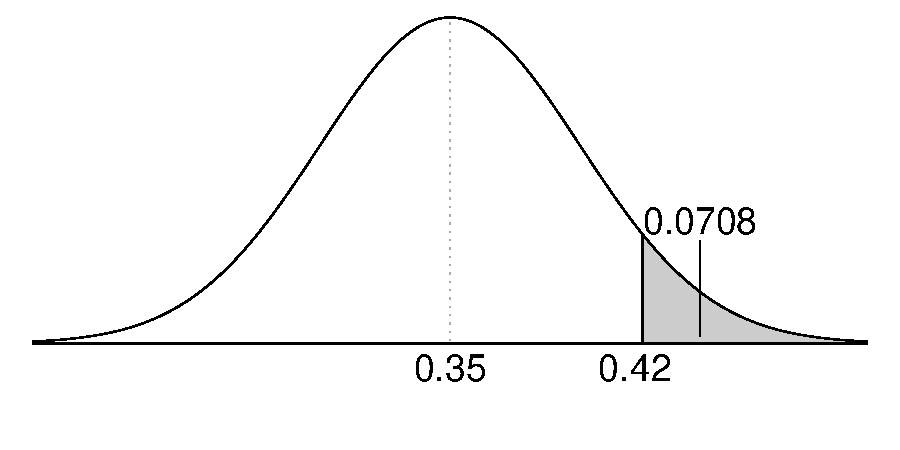
\includegraphics[width=70mm]{05/figures/eoce/abroad}
\end{center}
The data do not provide convincing evidence to suggest that the proportion of students at this university who have travelled abroad has increased after the implementation of the study abroad program.
\end{minipage}

\item If in fact 35\% of students at this university have travelled abroad, the probability of getting a random sample of 100 students where more than 42\% have travelled abroad is 0.0708.

\item Yes, we failed to reject the null hypothesis which claims $p = 0.35$ and this value is also included in the confidence interval.

\end{enumerate}

}

% 

{\dph{
\eoce{Is there strong evidence that the continental U.S. is warming? We might take a simple approach to this problem and compare how temperatures have changed from 1968 to 2008. In Exercise~\eoceref{temperatureWarming} we considered the differences between the temperature readings in January 1 of 1968 and 2008 at 51 locations in the continental US, but we might also consider the proportion of locations where a temperature increase was recorded between 1968 and 2008. It was observed that the January 1 temperature was warmer in 2008 for 32 of the 51 locations. Does this provide convincing evidence that January 1 temperatures in more than half of the US are warmer in 2008 than they were in 1968?
\begin{enumerate}[(a)]
\setlength{\itemsep}{0mm}
\item Write the hypotheses in symbols and in words.
\item Are assumptions and conditions for inference satisfied?
\item Calculate the test statistic.
\item Find and interpret the p-value in context.
\item Based on the hypothesis test, do the data suggest that January 1 temperatures in more than half of the US are warmer in 2008 than they were in 1968? Explain.
\end{enumerate}
}
{
\begin{enumerate}[(a)]
\item $H_0: p = 0.5$ (Temperatures in 50\% of locations in the continental US were warmer in 2008 than they were in 1968) \\
$H_A: p > 0.5$ (Temperatures in more than 50\% of locations in the continental US were warmer in 2008 than they were in 1968)
\item
\begin{enumerate}[1.]
\item Independence Assumption: 
\begin{itemize}
\item Random Sampling Condition: We are told that the locations are sampled randomly.
\item 10\% Condition: $51$ $<$ 10\% of all locations in the continental US.
\end{itemize}
Since we have a random sample and the 10\% condition is satisfied, we can assume that whether or not there was a temperature increase in one location in the sample is independent of another.
\item Nearly Normal Condition: First we must check if the success failure condition is met.
\begin{align*}
n\hat{p} &\ge 10 \rightarrow 51 * 0.5 = 20.5 > 10 \checkmark \\
n(1 - \hat{p}) &\ge 10 \rightarrow 51 * 0.5 = 20.5 > 10 \checkmark
\end{align*}
Since the observations are independent and the success-failure condition is met, we can assume that $\hat{p}$ is nearly normal.
\end{enumerate}
\item The test statistic can be calculated as follows:
\begin{align*}
\hat{p} &= \frac{32}{51} = 0.6275 \\
z &= \frac{\hat{p} - p_0}{\sqrt{\frac{p_0 (1 - p_0)}{n}}} = \frac{0.6275 - 0.5}{\sqrt{\frac{0.5 * 0.5}{51}}} = 1.82
\end{align*}
\item p-value = $P(\hat{p} >  0.6275 | p = 0.5) = P(z > 1.82) = 1 - 0.9656 = 0.0344$
If in fact in half of all locations in the continental US temperatures increased between January 1 1968 and 2008, the probability of getting a random sample of 51 locations where more than half had warmer temperatures in 2008 is 0.0344.
\item Since p-value $< \alpha$ (since not given use 0.05), we reject $H_0$. The data provide convincing evidence to suggest that January 1 temperatures in more than half of the US are warmer in 2008 than in 1968. It should be noted that using this approach we arrived at a different conclusion than we did in Exercise~\eoceref{temperatureWarming}.
\end{enumerate}
}
}}

%

\eoce{A college review magazine states that in many business schools there is a certain stigma that marketing is an easy major and that therefore majority of students majoring in marketing also major in finance, economics or accounting to be able to show employers that their quantitative skills are also strong. In order to test this claim an education researcher collects a random sample of 80 undergraduate students majoring in marketing at various business schools, and finds that 50 of them have a double major. Is there evidence to support the magazine's claim that majority of marketing students have a double major?
\begin{enumerate}[(a)]
\setlength{\itemsep}{0mm}
\item Write the hypotheses in symbols and in words.
\item Are assumptions and conditions for inference satisfied?
\item Calculate the test statistic.
\item Find and interpret the p-value in context.
\item Based on the hypothesis test, do the data suggest that majority of marketing students have a double major? Explain.
\end{enumerate}
}
{
\begin{enumerate}[(a)]
\item $H_0: p = 0.5$ (50\% of all marketing majors have a double major) \\
$H_A: p > 0.5$ (More than 50\% of all marketing majors have a double major)

\item
\begin{enumerate}[1.]
\item Independence Assumption: 
\begin{itemize}
\item Random Sampling Condition: We are told that the sample is random.
\item 10\% Condition: We can safely assume that $80$ $<$ 10\% of all undergraduate marketing majors.
\end{itemize}
Since we have a random sample and the 10\% condition is satisfied, we can assume that whether or not one student in the sample has a double major is independent of another.
\item Nearly Normal Condition: First we must check if the success failure condition is met.
\begin{align*}
n\hat{p} &\ge 10 \rightarrow 80 * 0.5 = 40 > 10 \checkmark \\
n(1 - \hat{p}) &\ge 10 \rightarrow 80 * 0.5 = 40 > 10 \checkmark
\end{align*}
Since the observations are independent and the success-failure condition is met, we can assume that $\hat{p}$ is nearly normal.
\end{enumerate}

\item The test statistic can be calculated as follows:
\begin{align*}
\hat{p} &= \frac{50}{80} = 0.625 \\
Z &= \frac{\hat{p} - p_0}{\sqrt{\frac{p_0 (1 - p_0)}{n}}} = \frac{0.625 - 0.5}{\sqrt{\frac{0.5 * 0.5}{80}}} = 2.24
\end{align*}

\item p-value = $P(\hat{p} > 0.625 | p = 0.5) = P(z > 2.24) = 1 - 0.9875 = 0.025$

If in fact half of all marketing students have a double major, the probability of getting a random sample of 80 marketing students where more than 50 have a double major is 0.025.
 
\item Since p-value $< \alpha$ (since not given use 0.05), we reject $H_0$. The data do not provide convincing evidence to suggest that majority of marketing students have a double major.
\end{enumerate}
}\label{DoubleMajor}

%

\eoce{Based on the information given in Exercise~\eoceref{DoubleMajor}, Construct a 90\% confidence interval for the proportion of marketing students who have a double major. Interpret this interval in context. Also comment on if the confidence interval agree with the conclusion of the hypothesis test from Exercise~\eoceref{DoubleMajor}. 
}
{
A 90\% confidence interval can be calculated as follows:
\begin{align*}
\hat{p} \pm z^* \sqrt{\frac{\hat{p} (1 - \hat{p})}{n}} &= 0.625 \pm 1.645 * \sqrt{\frac{0.625 * 0.375}{80}} \\
&= 0.625 \pm 0.089 \\
&= (0.54, 0.71)
\end{align*}
We are 90\% confident that the 54\% to 71\% of all undergraduate marketing students have a double major.

Yes, in Exercise~\eoceref{DoubleMajor} we rejected $H_0$ which claims that the population proportion equals 0.5 and the confidence interval does not include 0.5.
}

%

{\dph{
\eoce{A high school student is considering attending a nearby university. She is concerned that too many of the students attending the university live at home, and she has decided not to attend if there is strong evidence that more than 75\% of the registered students live at home.\\

\noindent The student experiences a fortunate coincidence. She recently finished a course in Advanced Placement Statistics, and the university student newspaper has published a poll of 400 randomly selected students at the university. 325 of these students reported that they still lived at home.
\begin{enumerate}[(a)]
\setlength{\itemsep}{0mm}
\item Write the hypotheses in symbols and in words to test whether more than 75\% of students at this college live at home. 
\item Are the assumptions and conditions for inference satisfied?
\item Calculate the test statistic.
\item Find and interpret the p-value in context.
\item Based on the hypothesis test do the data provide convincing evidence to suggest that more than 75\% of students at this college live at home? Explain.  Use $\alpha = 0.025.$
\end{enumerate}
}
{
\begin{enumerate}[(a)]
\item $H_0: p = 0.75$ (75\% of students at this college live at home) \\
$H_A: p > 0.75$ (More than 65\% of students at this college live at home)
\item
\begin{enumerate}[1.]
\item Independence Assumption: 
\begin{itemize}
\item Random Sampling Condition: We are told that the sample is random.
\item 10\% Condition: We can safely assume that 400 $<$ 10\% of all students at a college.
\end{itemize}
Since we have a random sample and the 10\% condition is satisfied, we can assume that whether or not one student in this sample lives at home is independent of another.
\item Nearly Normal Condition: First we must check if the success failure condition is met.
\begin{align*}
np &\ge 10 \rightarrow 400 * 0.75 = 300 > 10 \checkmark \\
n(1 - p) &\ge 10 \rightarrow 400 * 0.25 = 100 > 10 \checkmark
\end{align*}
Since the observations are independent and the success-failure condition is met, we can assume that $\hat{p}$ is nearly normal.
\end{enumerate}
\item The test statistic can be calculated as follows:
\begin{align*}
\hat{p} &= \frac{325}{1500} = 0.8125 \\
Z &= \frac{\hat{p} - p_0}{\sqrt{\frac{p_0 (1 - p_0)}{n}}} = \frac{0.8125 - 0.75}{\sqrt{0.75 * 0.25}{400}} = \frac{0.0625}{0.02165} = 2.89
\end{align*}
\item p-value = $P(\hat{p} > 0.8125 | p = 0.75) = P(z > 2.89) = 1 - 0.9981 = 0.0019 $ \\
$\:$ \\
If in fact 75\% of student at this college lived at home, the probability of getting a random sample of 400 students where more than 325 live at home would be 0.0019.
\item Yes, since p-value $< 0.025$, we reject $H_0$. The data provide convincing evidence to suggest that more than 75\% of students at this college live at home
\end{enumerate}
}\label{collegeStuLiveAtHome}
}}

%

{
\eoce{Using the data provided in Exercise~\eoceref{collegeStuLiveAtHome}, construct a 95\% confidence interval for the proportion of students at this college who live at home and interpret it in context. Does the conclusion of the hypothesis test from Exercise~\eoceref{collegeStuLiveAtHome} agree with the confidence interval?}
{
A 95\% confidence interval for the proportion of students at this college who live at home can be calculated as follows:
\begin{align*}
\hat{p} \pm z^* \sqrt{\frac{\hat{p} (1 - \hat{p})}{n}} &= 0.8125 \pm 1.96 * \sqrt{\frac{0.8125* 0.1875}{400}} \\
&= 0.8125 \pm 1.96 * 0.0195 \\
&= 0.8125 \pm 0.0382 \\
&= (0.7743 , 0.8507)
\end{align*}
We are 95\% confident that between approximately 77\% to 85\% of students at this college live at home. This interval agrees with the conclusion of the hypothesis test from Exercise~\eoceref{collegeStuLiveAtHome} since it lies above 75\%.
}
}

%

\eoce{A Washington Post article \citep{WashingtonPost} reports that ``a new Washington Post-ABC News poll shows that support for a government-run health-care plan to compete with private insurers has rebounded from its summertime lows and wins clear majority support from the public." More specifically the article says ``seven in 10 Democrats back the plan, while almost nine in 10 Republicans oppose it. Independents divide 52 percent against, 42 percent in favor of the legislation." There were were 819 Democrats, 566 Republicans and 783 independents surveyed. \\

\noindent A political pundit on TV claims that Democrats should not count on the independent votes for the public option plan since more than half of the independents oppose it. Is there significant evidence to support the pundit's claim?
\begin{enumerate}[(a)]
\setlength{\itemsep}{0mm}
\item Write the hypotheses in symbols and in words.
\item Are the assumptions and conditions for inference satisfied?
\item Calculate the test statistic.
\item Find and interpret the p-value in context.
\item Based on the hypothesis test is there significant evidence to suggest that more than half of the independents oppose the public option plan? Explain.
\item Would you expect a confidence interval for the proportion of independents who oppose the public option plan to include 0.5? Explain.
\end{enumerate}
}
{
\begin{enumerate}[(a)]

\item $H_0: p = 0.50$ (50\% of all independents are oppose the public option plan) \\
$H_A:  p > 0.50$ (More than 50\% of all independents are oppose the public option plan)

\item 
\begin{enumerate}[1.]
\item Independence Assumption: 
\begin{itemize}
\item Random Sampling Condition: We are told that the sample is random.
\item 10\% Condition: 783 $<$ 10\% of all independents.
\end{itemize}
Since we have a random sample and the 10\% condition is satisfied, we can assume that whether or not one independent opposes the plan is independent of whether or not another one does.
\item Nearly Normal Condition: First we must check if the success failure condition is met.
\begin{align*}
np &\ge 10 \rightarrow  783 * 0.50 = 391.5 > 10 \checkmark \\
n(1 - p) &\ge 10 \rightarrow 783 * 0.50 = 391.5 > 10 \checkmark
\end{align*}
Since the observations are independent and the success-failure condition is met, we can assume that $\hat{p}$ is nearly normal.
\end{enumerate}

\item The test statistic can be calculated as follows:
\begin{align*}
\hat{p} &= 0.52 \\
Z &= \frac{\hat{p} - p_0}{\sqrt{\frac{p_0q_0}{n}}} = \frac{0.52 - 0.50}{\sqrt{\frac{0.50 * 0.50}{783}}} = 1.12
\end{align*}

\item p-value = $P(z > 1.12) = 1 - 0.8686 = 0.1314$
If in fact 50\% of all independents oppose the public option plan, the probability of getting a sample of 783 independent where more than 52\% oppose the plan is 0.1314.

\item No, since p-value $> \alpha$ (use $\alpha = 0.05$ since not given) we fail to reject $H_0$. The data do not provide convincing evidence to suggest that more than half of all independents oppose the public option plan.

\item Yes, since we failed to reject $H_0$, which claims that the proportion of independents who oppose the public option plan equals 0.5, we would expect a confidence interval to include this value.

\end{enumerate}
}\label{WashPost}

%

\eoce{Exercise~\eoceref{WashPost} presents the results of a political poll on support for the public option plan.
\begin{enumerate}[(a)]
\setlength{\itemsep}{0mm}
\item Calculate a 90\% confidence interval for the proportion of independents who oppose the public option plan.
\item Interpret the confidence interval in context.
\item Does your interval agree with the result of your hypothesis test from Exercise~\eoceref{WashPost}? Explain.
\item If we wanted to limit the margin of error of a 90\% confidence interval to 1\%, how many independents would we need to survey?
\end{enumerate}
}
{
\begin{enumerate}[(a)]
\item A 90\% confidence interval can be calculated as follows:
\begin{align*}
\hat{p} \pm z^* \sqrt{\frac{\hat{p} ( 1 - \hat{p})}{n}} &= 0.52 \pm 1.645 *  \sqrt{\frac{0.52 * 0.48}{783}} \\
&= 0.52 \pm 0.03 \\
&= (0.49, 0.55)
\end{align*}

\item We are 90\% confident that 49\% to 55\% of independents oppose the public option plan.

\item Yes, we failed to reject $H_0$ and the interval includes 0.5.

\item  We are asked to solve for the sample size required to achieve a 1\% margin of error. 
\begin{align*}
ME = z^* \sqrt{ \frac{\hat{p} (1-\hat{p})} {n} } \rightarrow 0.01 &= 1.645 \sqrt{ \frac{0.52 * 0.48} {n} } \\
0.01^2 &= 1.645 ^2  \frac{0.52 * 0.48}{n} \\
n &= \frac{1.645 ^2 * 0.52 * 0.48}{0.01^2} \\
n &= 6754.238 \approx 6755
\end{align*}

\end{enumerate}
}

%

\edit{
\eoce{Some people claim that they can tell the difference between a diet soda and a regular soda in the first sip. A researcher wanting to test this claim randomly sampled 80 such people. He then filled 80 plain white cups with soda, half diet and half regular through random assignment, and asked each person to take one sip from their cup and identify the soda as ``diet" or ``regular". 53 participants correctly identified the soda. Does this suggest that these people are able to detect the difference between diet and regular soda, in other words, are the results significantly better than just random guessing? Do not forget to check that the assumptions and conditions for inference are satisfied.
}
{
\begin{align*}
H_0&: p = 0.5 \text{(Results are equivalent to randomly guessing)} \\
H_A&: p > 0.5 \text{(Results are better than just randomly guessing)}
\end{align*}
Before conducting the hypothesis test, we must first check that the assumptions and conditions for inference are satisfied.
\begin{enumerate}[1.]
\item Independence Assumption: 
\begin{itemize}
\item Random Sampling Condition: We are told that the sample is random.
\item 10\% Condition: We can safely assume that 80 $<$ 10\% of all people who claim they can correctly identify a soda as diet or regular.
\end{itemize}
Since we have a random sample and the 10\% condition is satisfied, we can assume that whether or not one person in the sample can identify a soda correctly in independent of another.
\item Nearly Normal Condition: First we must check if the success failure condition is met.
\begin{align*}
np &\ge 10 \rightarrow  80 * 0.5 = 40 > 10 \checkmark \\
n(1 - p) &\ge 10 \rightarrow 80 * 0.5 = 40 > 10 \checkmark
\end{align*}
Since the observations are independent and the success-failure condition is met, we can assume that $\hat{p}$ is nearly normal.
\end{enumerate}
The test statistic and the p-value can be calculated as follows:
\begin{align*}
\hat{p} &= \frac{53}{80} = 0.6625 \\
Z &= \frac{\hat{p} - p_0}{\sqrt{\frac{p_0 (1 - p_0)}{n}}} = \frac{0.6625 - 0.5}{\sqrt{\frac{0.5 \times 0.5}{80}}} = 2.91 \\
p-value &= P(\hat{p} > 0.6625 | p = 0.5) = P(z > 2.91) = 1 - 0.9982 = 0.0018
\end{align*}
Since p-value $< \alpha$ (use $\alpha = 0.05$ since not given), we reject the null hypothesis. There is sufficient evidence to suggest that the rate of correctly identifying a soda for these people is significantly better than just by random guessing.
}\label{sodaDietReg}
}

%

{
\eoce{Interpret in context what the p-value calculated in Exercise~\eoceref{sodaDietReg} means.}
{If in fact people cannot tell the difference between diet and regular soda and they randomly guess, the probability of getting a random sample of 80 people where 53 or more identify a soda correctly would be 0.0018.}
}

%

\edit{
\eoce{According to the Centers for Disease Control and Prevention, 30\% of Americans are habitually getting less than six hours of sleep a night - far less than the recommended seven to nine hours. New York is known as ``the city that never sleeps". In a random sample of 300 New Yorkers it was found that 105 of them get less than six hours of sleep a night. Is there significant evidence to suggest that the rate of sleep deprivation for New Yorkers is higher than the rate of sleep deprivation in the population at large? Do not forget to check that the assumptions and conditions for inference are satisfied.
}
{
\begin{align*}
H_0&: p = 0.3 \text{(30\% of New Yorkers are sleep deprived)} \\
H_A&: p > 0.3 \text{(More than 30\% of New Yorkers are sleep deprived)}
\end{align*}
Before conducting the hypothesis test, we must first check that the assumptions and conditions for inference are satisfied.
\begin{enumerate}[1.]
\item Independence Assumption: 
\begin{itemize}
\item Random Sampling Condition: We are told that the sample is random.
\item 10\% Condition: 300 $<$ 10\% of all New Yorkers.
\end{itemize}
Since we have a random sample and the 10\% condition is satisfied, we can assume that whether or not one New Yorker in the sample is sleep deprived is independent of another.
\item Nearly Normal Condition: First we must check if the success failure condition is met.
\begin{align*}
np_0 &\ge 10 \rightarrow 300 * 0.3 = 90 > 10 \checkmark \\
n(1 -p_0) &\ge 10 \rightarrow 300 * 0.7 = 210 > 10 \checkmark
\end{align*}
Since the observations are independent and the success-failure condition is met, we can assume that $\hat{p}$ is nearly normal.
\end{enumerate}
The test statistic and the p-value can be calculated as follows:
\begin{align*}
\hat{p} &= \frac{105}{300} = 0.35 \\
Z &= \frac{\hat{p} - p_0}{\sqrt{\frac{p_0 (1 - p_0)}{n}}} = \frac{0.35 - 0.3}{\sqrt{\frac{0.3 \times 0.7}{300}}} = 1.89
p-value &= P(\hat{p} > 0.35 | p = 0.3) = P(z > 1.89) = 1 - 0.9706 = 0.0294
\end{align*}
Since p-value $< \alpha$ (use $\alpha = 0.05$ since not given), we reject the null hypothesis. The data provide convincing evidence to suggest that the rate of sleep deprivation for New Yorkers is higher than the rate of sleep deprivation in the population at large.
}\label{NYsleepDeprived}
}

%

{
\eoce{Interpret in context what the p-value calculated in Exercise~\eoceref{NYsleepDeprived} means.}
{If in fact 30\% of New Yorkers are sleep deprived, the probability of getting a random sample of 300 New Yorkers where more than 105 are sleep deprived is 0.0294.}
}

%

\eoce{A survey conducted five years ago by the health center at the university mentioned in Exercise~\eoceref{UnivSmoke} showed that 18\% of the students smoked. 
\begin{enumerate}[(a)]
\setlength{\itemsep}{0mm}
\item Is there evidence to suggest that the percentage of students who smoke has changed over the last five years?
\item What type of error might we have committed above?
\end{enumerate}
}
{
\begin{enumerate}[(a)]

\item $H_0: p = 0.18$ (18\% of students at this university smoke) \\
$H_A: p \ne 0.18$ (More than 18\% of students at this university smoke) \\

We have already checked the assumptions and conditions necessary for inference in Exercise~\eoceref{UnivSmoke}. However we need to re-check the success failure condition since in hypothesis testing we use $p$ instead of $\hat{p}$ when checking this condition.
\[ 200 * 0.18 = 36 > 10 \checkmark \text{ and } 200 * 0.82 = 164 > 10 \checkmark \]
\begin{align*}
z &= \frac{0.20 - 0.18}{\sqrt{\frac{0.20 * 0.80}{200}}} = 0.71 \\
p-value &= P(\hat{p} < 0.16 \text{ OR } \hat{p} > 0.20 | p = 0.18) \\
&= 2 * P(z > 0.71) = 2 * (1 - 0.7611) = 2 * 0.2389 = 0.4778
\end{align*}

Since p-value $> \alpha$ (use $\alpha = 0.05$ since not given), we fail to reject the null hypothesis. The data do not provide convincing evidence to suggest that the percentage of students at this university who smoke has changed over the last five years.

\item Since we failed to reject the null hypothesis, we may have committed a Type II error.

\end{enumerate}
}

%

\edit{
\eoce{Michael Scott, a regional manager at Dunder Mifflin Paper Company, claims that over 45\% of businesses have Dunder Mifflin as their sole paper provider. To test his claim we randomly sampled 180 businesses and found that 36\% of these businesses had Dunder Mifflin as their sole paper provider. Is there significant evidence to support Michael Scott's claim that over 45\% of businesses have Dunder Mifflin as their sole paper provider?Do not forget to check that the assumptions and conditions for inference are satisfied.
}
{
\begin{align*}
H_0&:p = 0.45 \text{(45\% of businesses have Dunder Mifflin as their sole paper provider)} \\
H_A&:p > 0.45 \text{(More than 45\% of businesses have Dunder Mifflin as their sole paper provider)}
\end{align*}
Before conducting the hypothesis test, we must first check that the assumptions and conditions for inference are satisfied.
\begin{enumerate}[1.]
\item Independence Assumption: 
\begin{itemize}
\item Random Sampling Condition: We are told that the sample is random.
\item 10\% Condition: We can safely assume that 180 $<$ 10\% of all businesses.
\end{itemize}
Since we have a random sample and the 10\% condition is satisfied, we can assume that whether or not one business chooses Dunder Mifflin is independent of another.
\item Nearly Normal Condition: First we must check if the success failure condition is met.
\begin{align*}
np &\ge 10 \rightarrow 180 * 0.45 = 81 > 10 \checkmark \\
n(1 - p) &\ge 10 \rightarrow 180 * 0.55 = 99 > 10 \checkmark
\end{align*}
Since the observations are independent and the success-failure condition is met, we can assume that $\hat{p}$ is nearly normal.
\end{enumerate}
The test statistic and the p-value can be calculated as follows:
\begin{align*}
\hat{p} &= 0.36 \\
z &= \frac{\hat{p} - p_0}{\sqrt{\frac{p_0 (1 - p_0)}{n}}} = \frac{0.36 - 0.45}{\sqrt{\frac{0.45 * 0.55}{180}}} = -2.43 \\
p-value &= P(\hat{p} > 0.36 | p = 0.45) = P(z > -2.43) = 1 - 0.0075 = 0.9925
\end{align*}
Since p-value $> \alpha$ (use $\alpha = 0.05$ since $\alpha$ not given), we fail to reject $H_0$. There isn't sufficient evidence to support Michael Scott's claim that over 45\% of businesses have Dunder Mifflin as their sole paper provider.
}\label{dunderMifflin}
}

%

{
\eoce{Interpret in context what the p-value calculated in Exercise~\eoceref{NYsleepDeprived} means.}
{If in fact the true market share of Dunder Mifflin was 45\%, the probability of getting a sample of 180 businesses where 36\% or more of them have Dunder Mifflin as their sole paper provider would be 0.9925.}
}

%

\edit{
\eoce{Statistics show that traditionally about 65\% of Kansas residents go out of state for college. This year researchers wanting to see if this number has increased randomly sampled 1,500 high-school graduates and found that 1,005 went out of state for college. Based on these data is there strong evidence to suggest that the percentage of Kansas residents who go out of state for college has increased? Do not forget to check that the assumptions and conditions for inference are satisfied.
}
{
\begin{align*}
H_0&:p = 0.65 \text{(65\% of Kansas residents go out of state for college)} \\
H_A&: p > 0.65 \text{(More than 65\% of Kansas residents go out of state for college)}
\end{align*}
Before conducting the hypothesis test, we must first check that the assumptions and conditions for inference are satisfied.
\begin{enumerate}[1.]
\item Independence Assumption: 
\begin{itemize}
\item Random Sampling Condition: We are told that the sample is random.
\item 10\% Condition: We can safely assume that 1,500 $<$ 10\% of all Kansas high school graduates.
\end{itemize}
Since we have a random sample and the 10\% condition is satisfied, we can assume that whether or not one high school graduate goes out of state for college is independent of another.
\item Nearly Normal Condition: First we must check if the success failure condition is met.
\begin{align*}
np &\ge 10 \rightarrow 1500 * 0.65 = 975 > 10 \checkmark \\
n(1 - p) &\ge 10 \rightarrow 1500 * 0.35 = 525 > 10 \checkmark
\end{align*}
Since the observations are independent and the success-failure condition is met, we can assume that $\hat{p}$ is nearly normal.
\end{enumerate}
The test statistic and the p-value can be calculated as follows:
\begin{align*}
\hat{p} &= \frac{1005}{1500} = 0.67 \\
z &= \frac{\hat{p} - p_0}{\sqrt{\frac{p_0 (1 - p_0)}{n}}} = \frac{0.67 - 0.65}{\sqrt{0.65 * 0.35}{1500}} = 1.62 \\
p-value &= P(\hat{p} > 0.67 | p = 0.65) = P(z > 1.62) = 1 - 0.9474 = 0.0526
\end{align*}
Since p-value $> \alpha$ (use $\alpha = 0.05$ since not given), we fail to reject $H_0$. There isn't convincing evidence to suggest that the percentage of Kansas residents who go out of state for college has increased. It should however be noted that the p-value is very close to 0.05.
}\label{Kansas}
}

%

{
\eoce{Interpret in context what the p-value calculated in Exercise~\eoceref{Kansas} means.}
{If in fact 65\% Kansas residents went out of state for college, the probability of getting a sample of 1,500 Kansas residents where more than 1,005 go out of state for college would be 0.0526.}
}

%

{
\eoce{Hewes and Associates, a law firm in Manhattan, is investigating whether or not a chemical called aerocyte, used in mining operations by Ultima National Resources (UNR), increases the risk of certain types of cancer. Ellen Parsons, an associate at this firm, interviewed 300 randomly selected residents of counties where UNR has operations using aerocyte. Among these 27 had been diagnosed with stomach cancer. Based on research by the Centers for Disease Control it is known that among at risk populations 5\% will develop stomach cancer. Would you advise Hewes and Associates to proceed with the case, i.e. do the data provide convincing evidence that the rate of stomach cancer is higher among residents of counties where UNR has operations using aerocyte? Do not forget to check that the assumptions and conditions for inference are satisfied.
}
{
\begin{align*}
H_0: p = 0.05 &\text{(5\% of residents of counties where UNR has operations using} \\
&\text{aerocyte develop stomach cancer)} \\
H_A: p > 0.05 &\text{(More than 5\% of residents of counties where UNR has operations using} \\
&\text{aerocyte develop stomach cancer)}
\end{align*}
Before conducting the hypothesis test, we must first check that the assumptions and conditions for inference are satisfied.
\begin{enumerate}[1.]
\item Independence Assumption: 
\begin{itemize}
\item Random Sampling Condition:  The residents are randomly selected.
\item 10\% Condition: We can assume that 300 $<$ 10\% of all residents in counties where UNR has operations that uses aerocyte.
\end{itemize}
Since we have a random sample and the 10\% condition is satisfied, we can assume that whether or not one resident in this sample has stomach cancer is independent of another.
\item Nearly Normal Condition: First we must check if the success failure condition is met.
\begin{align*}
np &\ge 10 \rightarrow 300 * 0.05 = 15 > 10 \checkmark \\
n(1 - p) &\ge 10 \rightarrow 300 * 0.95 = 285 > 10 \checkmark
\end{align*}
Since the observations are independent and the success-failure condition is met, we can assume that $\hat{p}$ is nearly normal.
\end{enumerate}
The test statistic and the p-value can be calculated as follows:
\begin{align*}
\hat{p} &= \frac{27}{300} = 0.09 \\
z &= \frac{0.09 - 0.05}{ \sqrt{ \frac{0.05 * 0.95}{300} } } = \frac{0.04}{0.01258} = 3.18
p-value &= P(z > 3.18) = 1 - 0.9993 = 0.0007
\end{align*}
Since $p-value < \alpha$ (since not given use 0.05), reject $H_0$. The data provide convincing evidence to suggest that more than 5\% of residents of counties where UNR has operations using aerocyte develop stomach cancer.
}\label{aerocyte}
}

%

{
\eoce{Interpret in context what the p-value calculated in Exercise~\eoceref{aerocyte} means.}
{If in fact aerocyte is not not associated with a higher risk of stomach cancer, the probability of finding a random sample of 300 individuals where 9\% or more have stomach cancer is 0.0007.}
}

%

{
\eoce{Can the result of your hypothesis test from Exercise~\eoceref{aerocyte} be used to prove that aerocyte does/does not cause stomach cancer?
}
{
No, even though the hypothesis test showed an association since this is an observational study we cannot tell if there is a causal connection between exposure to areocyte and stomach cancer.
}
}

%

%%%
\subsection{Difference of two proportions}
%%%

\eoce{Exercise~\eoceref{Kansas} mentions that out of a randomly sample of 1,500 high-school graduates from Kansas 1,005 went out of state for college. A similar survey conducted in California shows that from a random sample of 1,250 California high-school graduates 600 went out of state for college.
\begin{enumerate}[(a)]
\setlength{\itemsep}{0mm}
\item Calculate a 90\% confidence interval for the difference between the population proportions of Kansas and California residents who go out of state for college. Do not forget to check that assumptions and conditions for inference are met.
\item Interpret the confidence interval in context.
\item Based on your confidence interval, is there significant evidence to suggest that a higher proportion of Kansas residents go out of state for college? Explain.
\item Could we use this interval as a proof that the college system is better in California and hence a higher proportion of California residents stay in the state for college? Explain.
\end{enumerate}
}
{
\begin{enumerate}[(a)]
\item Let Group 1 represent Kansas and Group 2 represent California. Then,
\[ \hat{p}_1 = 0.67 \hspace{20mm} \hat{p}_2 = \frac{600}{1250} = 0.48 \]
Before we can construct a confidence interval, we must first check that the assumptions and conditions are met.
\begin{enumerate}[1.]
\item Independence Assumption: 
\begin{itemize}
\item Random Sampling Condition: We are told that both samples are random.
\item 10\% Condition: We can safely assume that 1,500 $<$ 10\% of all Kansas high school graduates and 1,250 $<$ 10\% of all California high school graduates.
\end{itemize}
Since we have a random sample and the 10\% condition is satisfied, we can assume that whether or not one Kansas high school graduate goes out of state for college does depend on another and similarly whether or not one California high school graduate goes out of state for college does depend on another.
\item Nearly Normal Condition: First we must check if the success failure condition is met.
\begin{align*}
n_1p_1 &\ge 10 \rightarrow 1500 * 0.67 = 1005 > 10 \checkmark &\text{  and \hspace{2mm} } n_1(1 - p_1) &\ge 10 \rightarrow 1500 * 0.33 = 495 > 10 \checkmark \\
n_2p_2 &\ge 10 \rightarrow 1250 * 0.48 = 600 > 10 \checkmark &\text{  and \hspace{2mm} } n_2(1 - p_2) &\ge 10 \rightarrow 1250 * 0.52 = 650 > 10 \checkmark \\
\end{align*}
\item Independent Groups: The two samples are independent of each other.
\end{enumerate}

\begin{align*}
(\hat{p}_1 - \hat{p}_2) \pm z^*\sqrt{ \frac{\hat{p}_1 (1 - \hat{p}_1)}{n_1} + \frac{\hat{p}_2 (1 - \hat{p}_2)}{n_2} } &= (0.67 - 0.48) \pm 1.645 *  \sqrt{ \frac{0.67 * 0.33}{1500} + \frac{0.48 * 0.52}{1250} } \\
&= 0.19 \pm 0.03 \\
&= (0.16,0.22)
\end{align*}

\item We are 90\% confident that the true proportion of Kansas residents that go out of state for college is 16\% to 22\% higher than the true proportion of California residents who go out of state for college.

\item Yes, since the interval does not include 0.

\item No, this is an observational study. It does not tell us anything about the quality of the college system in California, and cannot be used to imply causation.

\end{enumerate}
}\label{KansasCaliHS}

%

\eoce{Exercise~\eoceref{KansasCaliHS} presents the results of two surveys conducted in Kansas and California. Conduct a hypothesis test to determine if there is a significant evidence to suggest that
\begin{enumerate}[(a)]
\setlength{\itemsep}{0mm}
\item a higher proportion of Kansas residents go out of state for college,
\item proportion of Kansas and California residents who go out of state for college are different.
\end{enumerate}
}
{
\begin{enumerate}[(a)]

\item Since we have already checked the assumptions and conditions necessary for inference in Exercise~\eoceref{KansasCaliHS}, we can proceed to the hypothesis test.
\begin{align*}
H_0: p_1 = p_2 &\text{ (Proportion of Kansas and California high school students who go out of state} \\
&\text{ for college are equal)} \\
H_A: p_1 > p_2 &\text{ (Proportion of Kansas and high school students who go out of state for college is} \\
&\text{ greater than that of California)}
\end{align*}
\begin{align*}
\hat{p} &= \frac{success_1 + success_2}{n_1 + n_2} = \frac{1005 + 600}{1500 + 1250} = \frac{1650}{2750} = 0.58 \\
z &= \frac{(\hat{p}_1 - \hat{p}_2) - (p_1 - p_2)}{\sqrt{ \frac{\hat{p} (1 - \hat{p})}{n_1} + \frac{\hat{p} (1 - \hat{p})}{n_2} }} = \frac{(0.67 - 0.48) - 0}{\sqrt{ \frac{0. 58 * 0.42}{1500} + \frac{0. 58 * 0.42}{1250} }} =  \frac{0.19}{0.0189} = 10.05 \\
p-value &= P((\hat{p}_1 - \hat{p}_2) > 0.19 | p_1 = p_2) = P(z > 10.05) \approx 0
\end{align*}

Since p-value is very small we reject $H_0$. There is sufficient evidence to suggest that proportion of Kansas and high school students who go out of state for college is greater than that of California. 

\item The hypotheses and the p-value changes, but the rest of the calculations are same as in part (a).
\begin{align*}
H_0: p_1 = p_2 &\text{ (Proportion of Kansas and California high school students who go out of state} \\
&\text{ for college are equal)} \\
H_A: p_1 \ne p_2 &\text{ (Proportion of Kansas and California high school students who go out of state} \\
&\text{ for college are different)}
\end{align*}
\[ p-value = P(| \hat{p}_1 - \hat{p}_2 | > 0.19 | p_1 = p_2) = 2 * P(z > 10.05) \approx 0 \]

Since p-value is still very small we reject $H_0$. There is sufficient evidence to suggest that proportion of Kansas and California high school students who go out of state for college are different.

\end{enumerate}
}

%

\eoce{Based on the information given in Exercise~\eoceref{WashPost}, is there significant evidence to suggest that a higher proportion of Democrats than independents support the public option plan?
\begin{enumerate}[(a)]
\setlength{\itemsep}{0mm}
\item Write the hypotheses in words and in symbols.
\item Calculate the test statistic.
\item Find the p-value and interpret it in context.
\item What do you conclude?
\item What type of error might we have committed?
\item Would you expect a confidence interval for the difference between the two proportions to include 0? Explain your reasoning. If you answered no, would you expect the confidence interval for $(p_{D} - p_{I})$ to be positive or negative?
\item Calculate a 90\% confidence interval for the difference between $(p_{D} - p_{I})$.
\item Interpret the confidence interval in context.
\item What does ``90\% confident" mean?
\item Does this imply that being a Democrat causes someone to support the public option plan? Explain.
\end{enumerate}
}
{
\begin{enumerate}[(a)]

\item Let $p_1$ denote the proportion of Democrats who support the plan and $p_2$ denote the proportion of independents who support the plan.
\begin{align*}
H_0: p_1 = p_2 &\text{ (Proportions of Democrats and independents who support the plan are equal.)} \\
H_A: p _1 > p_2 &\text{ (Proportion of Democrats who support the plan is higher than the proportion } \\
&\text{ of independents who support the plan.)}
\end{align*}

\item The test statistics can be calculated as follows:
\begin{align*}
&\hat{p}_1 = 0.70	&\hat{p}_2 = 0.42 \\
&n_1 = 819		&n_2 = 783
\end{align*}
\begin{align*}
success_1 &= n_1 \hat{p}_1 = 819 * 0.70 = 573.3 \approx 573 \\
success_2 &= n_2 \hat{p}_2 = 783 * 0.42 = 328.86 \approx 329 \\
\hat{p} &= \frac{success_1 + success_2}{n_1 + n_2} = \frac{579 + 329}{819 + 783} = \frac{908}{1602} \approx 0.57 \\
Z &= \frac{(\hat{p}_1 - \hat{p}_2)}{\sqrt{\frac{\hat{p} (1 - \hat{p})}{n_1} + \frac{\hat{p} (1 - \hat{p})}{n_2}}} = \frac{(0.70 - 0.42)}{\sqrt{\frac{0.57 * 0.43}{819} + \frac{0.57 * 0.43}{783}}} = 11.32
\end{align*}

\item p-value = $P(z > 11.32) \approx 0$. The probability of observing a $z$-statistic of 11.32 or higher given that the proportion of Democrats and independents who support the plan were equal is very low, almost 0.

\item Since p-value $<$ $\alpha$ (use $\alpha = 0.05$ since not given), we reject the null hypothesis. The data provide convincing evidence to suggest that the proportion of Democrats who support the plan is higher than the proportion of independents who support the plan.

\item Since we rejected the null hypothesis, we may have committed a Type I error.

\item No, rejecting the null hypothesis of $p_1 = p_2$ is equivalent to rejecting that $p_1 - p_2 = 0$. Therefore we would not expect a confidence interval for the difference between the two proportions to include 0. Since the alternative hypothesis that we are sticking with states that the proportion of Democrats who support the plan is higher than the proportion of independents who support the plan, we would expect the confidence interval for $(p_{D} - p_{I})$ to be positive.

\item A 90\% confidence interval can be calculated as follows:
\begin{align*}
(\hat{p}_1 - \hat{p}_2) \pm z^* \sqrt{ \frac{\hat{p}_1 (1 - \hat{p})_1}{n_1} + \frac{\hat{p}_2 (1 - \hat{p}_2)}{n_2} } &= (0.70 - 0.42) \pm 1.645 \sqrt{ \frac{0.70 * 0.30}{819} + \frac{0.42 * 0.58}{783} } \\
&= 0.28 \pm 0.04 \\
&= (0.24, 0.32)
\end{align*}

\item We are 90\% confident that the proportion of Democrats who support the plan is between 24\% and 32\% higher than the proportion of Independents who do.

\item 90\% of random samples of equivalent sizes will yield confidence interval that include the true difference between the population proportions of Democrats and Independents who support the plan.

\item No, based on the data we would conclude that there is a higher proportion of Democrats who support the public option plan than independents however we just cannot conclude that being a Democrat causes someone to support the public option plan as we cannot imply causation based on an observational study.
\end{enumerate}
}

%

\eoce{According to a report on sleep deprivation by the Centers for Disease Control and Prevention \citep{sleep} the proportion of California residents who reported insufficient rest or sleep during the on each of the preceding 30 days is 8.0\% while this proportion is 8.8\% for Oregon residents. A random sample of 11,545 California and 4,691 Oregon residents were surveyed. We are interested in finding out if there evidence to suggest that the rate of sleep deprivation is different for the two states.
\begin{enumerate}[(a)]
\setlength{\itemsep}{0mm}
\item What kind of study is this?
\item What are the hypotheses?
\item Are the assumptions and conditions for inference satisfied?
\item Calculate the test statistic.
\item Find and interpret the p-value in context.
\item What do you conclude? Interpret your conclusion in context.
\item Does this imply that the rate of sleep deprivation is equal in the two states? Explain.
\item What type of error might we have committed?
\item Would you expect a confidence interval for the difference between the two proportions to include 0? Explain your reasoning.
\end{enumerate}
}
{
\begin{enumerate}[(a)]

\item This is an observational study.

\item Let $p_1$ denote the proportion of sleep deprived California residents and $p_2$ denote the proportion of sleep deprived Oregon residents.
\begin{align*}
H_0: p_1 = p_2 \\
H_A: p_1 \ne p_2
\end{align*}

\item 
\begin{enumerate}[1.]
\item Independence Assumption: 
\begin{itemize}
\item Random Sampling Condition: We are told that both samples are random.
\item 10\% Condition: 11,545 $<$ 10\% of all Californians and 4,691 $<$ 10\% of all Oregonians.
\end{itemize}
Since we have a random sample and the 10\% condition is satisfied, we can assume that how much one Californian sleeps is independent of how much another Californian sleeps and how much one Oregonian sleeps is independent of how much another Oregonian sleeps.
\item Nearly Normal Condition: First we must check if the success failure condition is met.
\begin{align*}
n_1p_1 &\ge 10 \rightarrow 11,545 * 0.08 = 923.6 > 10 \checkmark &\text{  and \hspace{2mm} } n_1(1 - p_1) &\ge 10 \rightarrow 11,545 * 0.92 = 10621.4 > 10 \checkmark \\
n_2p_2 &\ge 10 \rightarrow 4,691 * 0.088 = 412.8 > 10 \checkmark &\text{  and \hspace{2mm} } n_2(1 - p_2) &\ge 10 \rightarrow 4,691 * 0.912 = 4278.2 > 10 \checkmark \\
\end{align*}
\item Independent Groups: The Californians and the Oregonians are independent of each other.
\end{enumerate}

\item The test statistic can be calculated as follows:
\begin{align*}
success_1 &= n_1 * p_1 = 11,545 * 0.08 = 923.6 \approx 924 \\
success_2 &= n_2 * p_2 = 4,691 * 0.088 = 412.8 \approx 413 \\
\hat{p}&= \frac{success_1 + success_2}{n_1 + n_2} = \frac{924 + 413}{11,545 + 4,691} = \frac{1,337}{16,236} \approx 0.082 \\
z &= \frac{(\hat{p}_1 - \hat{p}_2) - (p_1 - p_2)}{\sqrt{\frac{\hat{p} (1 - \hat{p}) }{n_1} + \frac{\hat{p} (1 - \hat{p})}{n_2}}} = \frac{(0.08 - 0.088) - 0}{\sqrt{\frac{0.082 * 0.918}{11,545} + \frac{0.082 * 0.918}{4,691}}} = -1.68
\end{align*}

\item p-value = $2 * P(z < -1.68) = 2 * 0.0465 = 0.093$

The probability of getting a z-statistic of -1.68 or lower or 1.68 or higher given that the proportion of Californians and Oregonians who are sleep deprived are equal is 0.093. In other words, the probability of getting a difference of 0.8\% or higher between the sample proportions of California and Oregon residents who are sleep deprived if in fact the two population proportions are equal is 0.093.

\item Since p-value $>$ $\alpha$ (use $\alpha = 0.05$ since not given), we fail to reject the null hypothesis and conclude that there is no evidence to suggest that the rate of sleep deprivation is different for the two states.

\item No, this does not imply it; though there is support for that statement. We cannot infer causation based on an observational study.

\item Since we failed to reject the null hypothesis, we may have committed a Type II error.

\item Yes, since we failed to reject the null hypothesis, it is possible that the two population proportions are equal to each other and hence the difference between them could be 0.

\end{enumerate}
}\label{OregonCaliSleepHT}

%

\eoce{Using the data provided in Exercise~\eoceref{OregonCaliSleepHT}, construct a 95\% confidence interval for the difference between the population proportions. Interpret the confidence interval in context.
}
{ A 95\% confidence interval for the difference between the population proportions can be calculated as follows:
\begin{align*}
&(\hat{p}_1 - \hat{p}_2) \pm z^* \sqrt{ \frac{\hat{p}_1 (1 - \hat{p}_1)}{n_1} + \frac{\hat{p}_2 (1 - \hat{p}_2)}{n_2} } \\
&= (0.08 - 0.088) \pm 1.96 \sqrt{ \frac{0.08 * 0.92}{11,545} + \frac{0.088 * 0.912}{4,691} } \\
&= -0.008 \pm 0.009 \\
&= (-0.017, 0.001)
\end{align*}

We are 95\% confident that the difference between the proportions of Californians and Oregonians who are sleep deprived is between -1.7\% and 0.1\%. In other words, we are 95\% confident that the proportion of Californians who are sleep deprives is 1.7\% less to 0.1\% more than the proportion of Oregonians who are sleep deprived.
}\label{OregonCaliSleepCI}

%

\eoce{Does the result of your hypothesis test from Exercise~\eoceref{OregonCaliSleepHT} agree with the interpretation of the confidence interval from Exercise~\eoceref{OregonCaliSleepCI}? If not, why might that be the case?}
{
This confidence interval from Exercise~\eoceref{OregonCaliSleepCI} includes 0 and we failed to reject the null hypothesis which set the two population proportions equal to each other in Exercise~\eoceref{OregonCaliSleepHT}, in other words sets the difference between the two population proportions to 0. So yes, the results of the hypothesis test and confidence interval agree.
}


% Distribution of the difference of two proportions

% Intervals and tests for p1 - p2

{
\eoce{A study published in 2001 asked 1924 male and 3666 female undergraduate college students their favorite color \citep{Ellis:2001}. A 95\% confidence interval for the difference between the proportions of males and females whose favorite color is black $(p_{male} - p_{female})$ was calculated to be (0.02, 0.06). Based on this information, determine if the following statements are true or false. Explain your reasoning.
\begin{enumerate}[(a)]
\setlength{\itemsep}{0mm}
\item We are 95\% confident that the true proportion of males whose favorite color is black is 2\% lower to 6\% higher than the true proportion of females whose favorite color is black.
\item We are 95\% confident that the true proportion of males whose favorite color is black is 2\% to 6\% higher than the true proportion of females whose favorite color is black.
%\item There is a 0.95 probability that the true difference between the population proportions of males and females whose favorite color is black is between 0.02 and 0.06.
\item 95\% of random samples will produce confidence intervals that include the true difference between the population proportions of males and females whose favorite color is black.
\item We can conclude that there is a significant difference between the proportions of males and females whose favorite color is black and that the difference between the two sample proportions was too large to plausibly be due to chance.
\item The 95\% confidence interval for $(p_{female} - p_{male})$ cannot be calculated without knowing the actual sample proportions.
\end{enumerate}
}
{
\begin{enumerate}[(a)]
\item FALSE. Since $(p_{male} - p_{female})$ is positive, proportion of males whose favorite color is black is higher than the proportion of females.
\item TRUE. This is the correct interpretation of the confidence interval.
%\item FALSE. ``95\% confident" is not a probability statement. The confidence interval either includes the true population mean or doesn't. 
\item TRUE. This is the correct interpretation of the confidence level.
\item TRUE. The confidence interval does not include 0.
\item FALSE. To get the 95\% confidence interval for $(p_{female} - p_{male})$ all we have to do is to swap the bounds of the confidence interval for $(p_{male} - p_{female})$ and take their negatives; (-0.06,-0.02).
\end{enumerate}
}
}

%

{
\eoce{Researchers studying the effectiveness of an anti-anxiety medication randomly sampled 100 patients diagnosed with general anxiety disorder (GAD). Through random assignment half of the patients received a placebo and the other half the anti-anxiety medication. The treatment was considered a \textit{success} if the patient experienced a reduction in their anxiety level. A 95\% confidence interval for the difference between the proportion of success in the two groups $(p_{medication} - p_{placebo})$ was (-0.02, 0.24). Based on this information, determine if the following statements are true or false. Explain your reasoning.
\begin{enumerate}[(a)]
\setlength{\itemsep}{0mm}
\item We are 95\% confident that the true proportion of success among the population of people who take the medication is 2\% lower to 24\% higher than the true proportion of success among the population of people who take a placebo.
\item 95\% of random samples will produce a difference between -0.02 and 0.24.
%\item There is a 0.95 probability that the true difference between the population proportions is between -0.02 and 0.24.
\item The 95\% confidence interval for $(p_{placebo} - p_{medication})$ cannot be calculated without knowing the actual sample proportions.
\item The 95\% confidence interval for $(p_{placebo} - p_{medication})$ would be (-0.24, 0.02).
\item We can conclude that the medication was effective and the difference between the two sample proportions was too large to plausibly be due to chance.
\end{enumerate}
}
{
\begin{enumerate}[(a)]
\item TRUE. This is the correct interpretation of the confidence interval.
\item FALSE. Based on the confidence interval we cannot make inference about sample statistics.
%\item FALSE. ``95\% confident" is not a probability statement. The confidence interval either includes the true population mean or doesn't.
\item FALSE. To get the 95\% confidence interval for $(p_{placebo} - p_{medication})$ all we have to do is to swap the bounds of the original confidence interval and take their negatives.
\item TRUE. This is the correct confidence interval for $(p_{placebo} - p_{medication})$.
\item FALSE. The confidence interval for the difference between the proportions of success includes 0, therefore the true difference between the population proportions might be equal to 0, which means that the observed difference between the two sample proportions could be due to chance. 
\end{enumerate}
}
}

% Hypothesis testing when H0: p1 = p2

{
\eoce{In a survey conducted by Survey USA on July 12, 2010, 827 registered voters in California were asked ``Do you support? Or do you oppose? drilling for oil and natural gas off the Coast of California? Or do you not know enough to say?" Below is the distribution of responses based on whether or not the respondent graduated from college. We might expect that college graduates would be more likely to have an opinion on this issue than non-college graduates. Therefore we are interested in finding out if the proportion of college graduates who do not have an opinion on the matter, i.e. responded ``do not know", is lower than the proportion of non-college graduates who do not have an opinion on the matter. \vspace{1mm}\\
\begin{minipage}[c]{0.48\textwidth}
\begin{enumerate}[(a)]
\setlength{\itemsep}{0mm}
\item What percent college the graduates and what percent of the non-college graduates in this sample do not know enough to have an opinion on drilling for oil and natural gas off the Coast of California?
\item Write the appropriate hypotheses. 
\item Calculate the test statistic and the p-value.
\item What is the conclusion of the hypothesis test? Interpret your conclusion in context.
\end{enumerate}
\end{minipage}
\begin{minipage}[c]{0.49\textwidth}
\begin{center}
\begin{tabular}{l l c c}
				&			& \multicolumn{2}{c}{\textit{College Grad}} \\
\cline{3-4}
				&			& Yes		& No				\\
\cline{2-4}
				& Support		& 154		& 132			\\
\textit{Response}	& Oppose		& 180		& 126			\\
				& Do not know	& 104		& 131			\\
\cline{2-4}
				& Total		& 438		& 389		
\end{tabular}
\end{center}
\end{minipage}
}
{
\begin{enumerate}[(a)]
\item The percentages can be calculated as follows:
\begin{align*}
&P(Do~not~know | College~Grad) = \frac{104}{438} = 0.237 \rightarrow 23.7\% \\
&P(Do~not~know | Non~College~Grad) = \frac{131}{389} = 0.337 \rightarrow 33.7\%
\end{align*}
\item Let college graduates be group 1 and non-college graduates be group 2.
\begin{align*}
H_0&: p_1 = p_2 \\
H_A&: p_1 < p_2
\end{align*}
\item The test statistic and the p-value can be calculated as follows:
\begin{align*}
\hat{p} &= \frac{104 + 131}{438 + 389} = \frac{235}{827} = 0.284 \\
\hat{q} &= 1 - 0.346 =  0.716 \\
Z &= \frac{\hat{p}_1 - \hat{p}_2}{\sqrt{ \frac{\hat{p}  \hat{q} }{n_1} + \frac{\hat{p} \hat{q} }{n_2} } } =  \frac{0.237 - 0.337}{\sqrt{ \frac{0.284  * 0.716 }{438} + \frac{ 0.284  * 0.716 }{389} } } = \frac{-0.1}{0.0314} = -3.18 \\
p-value &=  P(z < -3.18) = 0.0007
\end{align*}
\item Since p-value $< \alpha$ (0.05), we reject $H_0$. The data provide convincing evidence to suggest that the proportion of college graduates who responded do not know is lower than the proportion of non-college graduates who responded do not know.
\end{enumerate}
}\label{drillBabyDrill}
}

%

\eoce{Based on the data given in Exercise~\eoceref{drillBabyDrill} we are interested in finding out if there is a significant difference between the proportions of college graduate and non-college graduate California voters who support drilling for oil and natural gas off the Coast of California.
\begin{enumerate}[(a)]
\setlength{\itemsep}{0mm}
\item What percent college the graduates and what percent of the non-college graduates in this sample support drilling for oil and natural gas off the Coast of California?
\item Write the appropriate hypotheses. 
\item Calculate the test statistic and the p-value.
\item What is the conclusion of the hypothesis test? Interpret your conclusion in context.
\end{enumerate}
}
{
\begin{enumerate}[(a)]
\item The percentages can be calculated as follows:
\begin{align*}
&P(Support | College~Grad) = \frac{154}{438} = 0.352 \\
&P(Support | Non~College~Grad) = \frac{132}{389} = 0.339
\end{align*}
\item Let college graduates be group 1 and non-college graduates be group 2.
\begin{align*}
H_0&: p_1 = p_2 \\
H_A&: p_1 \ne p_2
\end{align*}
\item The test statistic and the p-value can be calculated as follows:
\begin{align*}
\hat{p} &= \frac{154 + 132}{438 + 389} = \frac{286}{827} = 0.346 \\
\hat{q} &= 1 - 0.346 =  0.654 \\
z &= \frac{\hat{p}_1 - \hat{p}_2}{\sqrt{ \frac{\hat{p}  \hat{q} }{n_1} + \frac{\hat{p} \hat{q} }{n_2} } } =  \frac{0.352 - 0.339}{\sqrt{ \frac{0.346  * 0.654 }{438} + \frac{ 0.346  * 0.654 }{389} } } = \frac{0.013}{0.033} = 0.39 \\
p-value &= P(|z| > 0.39) = P(z < -0.39) + P(z > 0.39) = 0.3483 + 0.3483 = 0.6966
\end{align*}
\item Since p-value $> \alpha$ (0.05), we fail to reject $H_0$. There isn't convincing evidence to suggest that there is a significant difference between the proportions of college graduate and non-college graduate California voters who support drilling for oil and natural gas off the Coast of California.
\end{enumerate}
}

%

{
\eoce{A CBS News article reports that ``Americans have differing views on two potentially inconvenient and invasive practices that airports could implement to uncover potential terrorist attacks." \citep{CBSPoll} This news piece was based on a survey conducted among among a random sample of 1,137 adults nationwide, interviewed by telephone between November 7-10, 2010, where one of the questions on the survey was ``Some airports are now using ``full-body" digital x-ray machines to electronically screen passengers in airport security lines. Do you think these new x-ray machines should or should not be used at airports?"
Below is a breakdown of answers based on party affiliation:
\begin{center}
\begin{tabular}{ll  cc c} 
			&				& \multicolumn{3}{c}{\textit{Party Affiliation}} \\
\cline{3-5}
							&					& Republican 	& Democrat 	& Independent	\\
\cline{2-5}
\multirow{3}{*}{\textit{Answer}}		&Should				& 264	 	& 299		& 351 	\\
							&Should not			& 38	 		& 55 	 		& 77 \\
							&Don't know/No answer	& 16	 		& 15 	 		& 22 \\
\cline{2-5}
							&Total				& 318		& 369		& 450
\end{tabular}
\end{center}
Based on these data, is there convincing evidence to suggest that there is a difference in opinion between Republicans and Democrats on the use of full-body scans, i.e. are proportions of Republicans and Democrats who think full-body scans should be used at airports are significantly different?
\begin{enumerate}[(a)]
\setlength{\itemsep}{0mm}
\item Write the hypotheses in words and in symbols.
\item Calculate the test statistic.
\item Find the p-value and interpret it in context.
\item What do you conclude?
\item What type of error might we have committed?
\item Would you expect a confidence interval for the difference between the two proportions to include 0? Explain your reasoning.
\end{enumerate}
}
{
\begin{enumerate}[(a)]
\item Let $p_1$ denote the proportion of Republicans who support the use of full-body scans and $p_2$ denote the proportion of Democrats who support the use of full-body scans
\begin{align*}
H_0: p_1 = p_2 &\text{ (Proportions of Republicans and Democrats who support the use of full-body} \\
&\text{scans are equal.)} \\
H_A: p _1 \ne p_2 &\text{ (Proportions of Republicans and Democrats who support the use of full-body} \\
&\text{scans are different.)}
\end{align*}
\item The test statistic can be calculated as follows:
\begin{align*}
&success_1 = 264				&success_2 = 299 \\
&n_1 = 318					&n_2 = 369 \\
&\hat{p}_1 = \frac{264}{318} = 0.83	&\hat{p}_2 = \frac{299}{369} = 0.81 \\
\end{align*}
\begin{align*}
\hat{p} &= \frac{success_1 + success_2}{n_1 + n_2} = \frac{264 + 299}{318 + 369} = \frac{563}{687} \approx 0.82 \\
z &= \frac{(\hat{p}_1 - \hat{p}_2)}{\sqrt{\frac{\hat{p} \hat{q}}{n_1} + \frac{\hat{p} \hat{q}}{n_2}}} = \frac{(0.83 - 0.81)}{\sqrt{\frac{0.82 * 0.18}{318} + \frac{0.82 * 0.18}{369}}} = \frac{0.02}{0.0294} = 0.68
\end{align*}
\item p-value = $P(|z| > 0.68) = 0.2483 + 0.2483 = 0.4966 $. 
$\:$ \\
If in fact the proportions of Republicans and Democrats who support the use of full-body scans at airports were equal, the probability of getting a random sample of 318 Republicans and 318 Democrats where difference between the proportions in these samples is 2\% or higher would be 0.4966.
\item Since p-value $>$ $\alpha$ (use $\alpha = 0.05$ since not given), we fail to reject the null hypothesis and conclude that there isn't convincing evidence to suggest that the proportions of Republicans and Democrats who support the use of full-body scans are different.
\item Since we failed to reject the null hypothesis, we may have committed a Type II error.
\item Yes, since we failed to reject the null hypothesis of $p_1 = p_2$ (or said differently, $p_1 - p_2 = 0$), we would expect the confidence interval to include 0.
\end{enumerate}
}\label{fullBodyScan}
}

%

{
\eoce{Exercise~\eoceref{fullBodyScan} presents the results of a CBS News poll on public opinion on the use of full body scans at airports.
\begin{enumerate}[(a)]
\setlength{\itemsep}{0mm}
\item Calculate a 90\% confidence interval for the difference between the proportion Republicans and Democrats who support the use of full-body scans at airports.
\item Interpret the confidence interval in context.
\item What does 90\% confident mean?
\item Does this prove that a there is no difference in opinion on the use of full-body scans between Republicans and Democrats? Explain.
\end{enumerate}
}
{
\begin{enumerate}[(a)]
\item A 90\% confidence interval can be calculated as follows:
\begin{align*}
&(\hat{p}_1 - \hat{p}_2) \pm z^* \sqrt{ \frac{\hat{p}_1 \hat{q}_1}{n_1} + \frac{\hat{p}_2 \hat{p}_2}{n_2} } \\
&= (0.83 - 0.81) \pm 1.645 \sqrt{ \frac{0.83 * 0.17}{318} + \frac{0.81 * 0.19}{369} } \\
&= 0.02 \pm 1.645 * 0.0293 \\
&= 0.02 \pm 0.05 \\
&= (-0.03, 0.07)
\end{align*}
\item We are 90\% confident that the proportion of Republicans who support the use of full-body scans at airports is 3\% lower to 7\% higher than the proportion of Democrats who do.
\item 90\% of random samples of 318 Republicans and 369 Democrats would produce confidence intervals that include the true difference between the proportions of Republicans and Democrats support the use of full-body scans at airports.
\item No, this does not prove it; though the data does not provide convincing evidence to the contrary.
\end{enumerate}
}
}

%

\subsection{One-way tables and the chi-square distribution}

{
\eoce{A professor using an open-source introductory statistics book predicts that 60\% of the students will purchase a hard copy of the book, 25\% will print it out from the web, and 15\% will read it online. At the end of the semester she asks her students to complete a survey where they indicate what format of the book they used. Of the 126 students, 71 said they bought a hard copy of the book, 30 said they printed it out from the web, and 25 said they read it online.
\begin{enumerate}[(a)]
\setlength{\itemsep}{0mm}
\item State the hypotheses for testing if the professor's predictions were inaccurate.
\item Assuming that the professor's predictions were correct, calculate the expected number of students who buy a hard copy of the book, who print it out from the web, and who read it online.
\item Are the assumptions and conditions for inference satisfied?
\item Calculate the chi-squared statistic, the degrees of freedom associated with it, and the p-value.
\item Based on the p-value calculated in part (d), what is the conclusion of the hypothesis test? Interpret your conclusion in context.
\end{enumerate}
}
{
\begin{enumerate}[(a)]
\item $H_0$: The distribution of the format of the book used by the students follows the professor's predictions. \\
$H_A$: The distribution of the format of the book used by the students does not follow the professor's predictions.
\item $E_{hard~copy} = 126 * 0.60 = 75.6$ \\
$E_{print} = 126 * 0.25 = 31.5$ \\
$E_{online} = 126 * 0.15 = 18.9$
\item \begin{enumerate}[1.]
\item Independence Assumption: 
\begin{itemize}
\item Random Sampling Condition: We are not told explicitly that the sample is random however we have no reason to believe that this class is not representative of all introductory statistics students.
\item 10\% Condition: We can safely assume that 126 $<$ 10\% of all introductory statistics students.
\end{itemize}
Assuming random samples and with the 10\% condition is satisfied, we can assume that whether or not one student will purchase a hard copy of the book, print it our from the web or read it online is independent of another.
\item Large enough sample size: All expected counts are at least 10.
\item Format of the book used is a categorical variable.
\end{enumerate}
\item The chi-squared statistic, the degrees of freedom associated with it, and the p-value can be calculated as follows:
\begin{align*}
\chi^2 &= \sum \frac{(O - E)^2}{E} =  \frac{(71 - 75.6)^2} {75.6} + \frac{(30 - 31.5)^2} {31.5} + \frac{(25 - 18.9)^2} {18.9} = 2.32 \\
df &= k - 1 = 3 - 1 = 2 \\
0.01 &< p-value < 0.02
\end{align*}
\item Since p-value $< \alpha$, we reject $H_0$. There is convincing evidence to suggest that the distribution of the format of the book used by the students does not follow the professor's predictions, i.e. the professor seems to be off in her predictions.
\end{enumerate}
}
}

%

{
\eoce{A Gallup poll, released December 17, 2010, reveals that 40 percent of Americans believe that humans were created by God within the last 10,000 year \citep{CreationismGallup}. The article which also notes that belief in evolutionary origins of humans is slowly rising is based on the results of a survey that asked the following question:
\begin{adjustwidth}{2em}{2em}
``Which of the following statements comes closest to your views on the origin and development of human beings: (1) Human beings have developed over millions of years from less advanced forms of life, but God guided this process, (2) Human beings have developed over millions of years from less advanced forms of life, but God had no part in this process, (3) God created human beings pretty much in their present form at one time within the last 10,000 years or so?"
\end{adjustwidth}
Results were based on telephone interviews conducted December 10-12, 2010 with a random sample of 1,019 adults, aged 18 and over, living in the continental U.S., selected using random-digit dial sampling. The table below shows the distribution of responses (in percentages) from 2010 as well as from 2001 when a similar survey was conducted.
\begin{center}
\begin{tabular}{l c c}
											& \multicolumn{2}{c}{\textit{Year}} \\
\cline{2-3}
\textit{Response}								& 2010	& 2001 \\
\hline
Humans evolved, with God guiding (1)				& 38\% 	& 37\% \\
Humans evolved, but God had no part in process (2) 	& 16\% 	& 12\% \\
God created humans  in present form (3) 				& 40\% 	& 45\% \\
Other / No opinion (4)							& 6\% 	& 6\% \\
\end{tabular}
\end{center} 
\begin{enumerate}[(a)]
\setlength{\itemsep}{0mm}
\item Calculate the actual number of respondents in 2010 that fall in each response category.
\item State the null and alternative hypotheses for testing if the distribution of the belief in evolutionary origins of humans has changed from 2001 to 2010.
\item Assuming that the distribution of the belief in evolutionary origins of humans has not changed from 2001 to 2010, calculate the expected number of respondents in 2010 that fall in each response category.
\item Are the assumptions and conditions for inference satisfied?
\item Calculate the chi-squared statistic, the degrees of freedom associated with it, and the p-value.
\item Based on the p-value calculated in part (e), what is the conclusion of the hypothesis test? Interpret your conclusion in context. 
\item Does the conclusion of the hypothesis test support the comment that ``belief in evolutionary origins of humans is slowly rising"?
\end{enumerate}
}
{
\begin{enumerate}[(a)]
\item $O_{(1)} = 1,019 * 0.38 = 387$ \\
$O_{(2)} = 1,019 * 0.16 = 163$ \\
$O_{(3)} = 1,019 * 0.40= 408$ \\
$O_{(4)} = 1,019 * 0.06 = 61$
\item $H_0$: Distribution of the belief in evolutionary origins of humans has not changed from 2001 to 2010. \\
$H_A$: Distribution of the belief in evolutionary origins of humans has changed from 2001 to 2010.
\item  $E_{(1)} = 1,019 * 0.37 = 377$ \\
$E_{(2)} = 1,019 * 0.12 = 122$ \\
$E_{(3)} = 1,019 * 0.45= 459$ \\
$E_{(4)} = 1,019 * 0.06 = 61$
\item \begin{enumerate}[1.]
\item Independence Assumption: 
\begin{itemize}
\item Random Sampling Condition: We are told that the sample is random.
\item 10\% Condition: 1,019 $<$ 10\% of all Americans.
\end{itemize}
Since we have a random sample and the 10\% condition is satisfied, we can assume that respondents' answers are independent of each other.
\item Large enough sample size: All expected counts are at least 10.
\item Response is a categorical variable.
\end{enumerate}
\item The chi-squared statistic, the degrees of freedom associated with it, and the p-value can be calculated as follows:
\begin{align*}
\chi^2 &= \sum \frac{(O - E)^2}{E} =  \frac{(387 - 377)^2} {377} + \frac{(163 - 122)^2} {122} + \frac{(408 - 459)^2} {459} + \frac{(61 - 61)^2}{61} = 19.71 \\
df &= k - 1 = 4 - 1 = 3 \\
p-value &< 0.001
\end{align*}
\item Since p-value $< \alpha$, we reject $H_0$. There is convincing evidence to suggest that the distribution of the belief in evolutionary origins of humans has changed from 2001 to 2010. Since an increase was observed in the response ``Humans evolved, but God had no part in process" there is support for the comment.
\end{enumerate}
}
}


%

\subsection{Two-way tables and chi-square}

{
\eoce{Exercise~\eoceref{fullBodyScan} presents the results of a CBS News poll on public opinion on the use of full body scans at airports. Based on these data, if in fact party affiliation is independent of support for the use of full-body scans, 
\begin{enumerate}[(a)]
\setlength{\itemsep}{0mm}
\item how many republicans would you expect to not support the use of full-body scans, 
\item how many democrats would you expect to support the use of full-body scans, and
\item how many independents would you expect to not know or not answer?
\end{enumerate}
}
{
\begin{enumerate}[(a)]
\item $E_{row_2, col_1} = \frac{(row~2~total)*(col~1~total)}{table~total} = \frac{(38+55+77) * 318}{(318+369+450)} = \frac{170 * 318}{1137} = 47.5$
\item $E_{row_1, col_2} = \frac{(row~1~total)*(col~2~total)}{table~total} = \frac{(264+299+351) * 369}{1137} = \frac{914 * 369}{1137} = 296.6$
\item $E_{row_3, col_3} = \frac{(row~3~total)*(col~3~total)}{table~total} = \frac{(16+15+22) * 450}{1137} = \frac{53 * 450}{1137} = 21.0$
\end{enumerate}
}
}

%

{
\eoce{Exercise~\eoceref{KansasCaliHS} presents the results of two surveys conducted in Kansas and California. 
\begin{enumerate}[(a)]
\setlength{\itemsep}{0mm}
\item Create a two-way table presenting the results of these two surveys.
\item If in fact there was no difference between the true proportions of Kansas and California high-school students who go out of state for college, how many students from each state would be expected to go out of state for college?
\end{enumerate}
}
{
\begin{enumerate}[(a)]
\item Below is a two-way table presenting the results of these two surveys:
\begin{center}
\begin{tabular}{l l c c c}
								&			& \multicolumn{2}{c}{\textit{Went out of state}}	&		\\
\cline{3-4}
								&			& Yes		& No		& Total	\\
\cline{2-5}
\multirow{2}{*}{\textit{State	}}		& Kansas		& 1,005		& 495	& 1,500	\\
								& California	& 600		& 650	& 1,250	\\
\cline{2-5}
								& Total		& 1,605		& 1,145	& 2,750
\end{tabular}
\end{center} 
\item Expected number of Kansas students who go out of state for college:
\[ E_{row~1, col~1} = \frac{(row~1~total)*(col~1~total)}{table~total} = \frac{1,500 * 1,605}{2,750} = 875.5 \]
Expected number of California students who go out of state for college:
\[ E_{row~2, col~1} = \frac{(row~2~total)*(col~1~total)}{table~total} = \frac{1,250 * 1,605}{2,750} = 729.5 \]
\end{enumerate}
}
}

%

{\dph{
\eoce{In July 2008 the US National Institutes of Health announced that it was stopping a clinical study early because of unexpected results.  The study population consisted of HIV-infected women in sub-Saharan Africa who had been given single dose Nevaripine (a treatment for HIV) while giving birth, to prevent transmission of HIV to the infant.  The study was a randomized comparison of continued treatment of a woman (after successful childbirth) with Nevaripine vs. Lopinavir, a second drug used to treat HIV.\\
$\:$ \\
240 women participated in the study; 120 were randomized to each of the two treatments. Twenty-four weeks after starting the study treatment, each woman was tested to determine if the HIV infection was becoming worse (an outcome called virologic failure). Twenty-six of the 120 women treated with Nevaripine experienced virologic failure, while 10 of the 120 women treated with the other drug experienced virologic failure.
\begin{enumerate}[(a)]
\setlength{\itemsep}{0mm}
\item Create a two-way table presenting the results of this study.
\item State the null and alternative hypotheses for testing for independence of treatment and virologic failure.
\item Calculate the expected number of observations for each of the cells under the null hypothesis.
\item Are the assumptions and conditions for inference satisfied?
\item Calculate the chi-squared statistic, the degrees of freedom associated with it, and the p-value.
\item Based on the p-value calculated in part (c), what is the conclusion of the hypothesis test? Interpret your conclusion in context.
\end{enumerate}
}
{
\begin{enumerate}[(a)]
\item The below two-way table presents the results of this study:
\begin{center}
\begin{tabular}{l l c c c}
								&			& \multicolumn{2}{c}{\textit{Virol. failure}}	&		\\
\cline{3-4}
								&			& Yes		& No		& Total	\\
\cline{2-5}
\multirow{2}{*}{\textit{Treatment}}		& Nevaripine	& 26			& 94		& 120	\\
								& Lopinavir	& 10			& 110	& 120	\\
\cline{2-5}
								& Total		& 36			& 204	& 240
\end{tabular}
\end{center} 
\item $H_0$: There is no difference in virologic failure rates between the Nevaripine and Lopinavir groups. \\
$H_A$: There is some difference in virologic failure rates between the Nevaripine and Lopinavir groups.
\item The expected counts can be calculated as follows:
\begin{align*}
E_{row~1, col~1} &= \frac{(row~1~total)*(col~1~total)}{table~total} = \frac{120 * 36}{240} = 18 \\
E_{row~1, col~2} &= \frac{(row~1~total)*(col~2~total)}{table~total} = \frac{120 * 204}{240} = 102 \\
E_{row~2, col~1} &= \frac{(row~2~total)*(col~1~total)}{table~total} = \frac{120 * 36}{240} = 18 \\
E_{row~2, col~2} &= \frac{(row~2~total)*(col~2~total)}{table~total} = \frac{120 * 204}{240} = 102
\end{align*}
\item \begin{enumerate}[1.]
\item Independence Assumption: 
\begin{itemize}
\item Random Sampling Condition: We are not told that the sample is random however random assignment was used.
\item 10\% Condition: We can safely assume that 120 $<$ 10\% of all HIV-infected women in sub-Saharan Africa who do and who do not experience virologic failure.
\end{itemize}
Since we have a random sample and with the 10\% condition is satisfied, we can assume that whether or not one woman in the sample experiences virologic failure is independent of another.
\item Large enough sample size: All expected counts are at least 10.
\item Treatment and virologic failure are both categorical variables.
\end{enumerate}
\item The chi-squared statistic, the degrees of freedom associated with it, and the p-value can be calculated as follows:
\begin{align*}
\chi^2 &= \sum \frac{(O - E)^2}{E} =  \frac{(26 - 18)^2} {18} + \frac{(24 - 102)^2} {102} + \frac{(20 - 18)^2} {18} + \frac{(110 - 102)^2} {102} = 8.37 \\
df &= (R - 1) * (C - 1) = (2 - 1) * (2 - 1) = 1 \\
0.001 &< p-value < 0.005
\end{align*}
\item Since p-value $< \alpha$, we reject $H_0$. There is convincing evidence to suggest a difference in virologic failure rates between the Nevaripine and Lopinavir groups, i.e treatment and virologic failure do not appear to be independent.
\end{enumerate}
}
}}

%

{\dph{
\eoce{Does smoking delay conception? The data in the table below are modeled after data obtained in an observational study comparing time to conception among women who were smokers with times for non-smoking women. Researchers asked a random sample of women who were pregnant with planned pregnancies how long it took them to become pregnant. Length of time to pregnancy was measured by the number of menstrual cycles between stopping birth control and getting pregnant. The women in the study were classified according to whether they were smokers or non-smokers, and whether they become pregnant during their first cycle.
\begin{center}
\begin{tabular}{l l c c c}
								&			& \multicolumn{2}{c}{\textit{Pregnancy occurred after}}	&		\\
\cline{3-4}
								&			& First cycle	& Two or more cycles		& Total	\\
\cline{2-5}
\textit{Smoking}						& Smoker		& 15			& 45						& 60	\\
\textit{status}						& Non-smoker	& 100		& 150					& 250	\\
\cline{2-5}
								& Total		& 115		& 195					& 310
\end{tabular}
\end{center} 
\begin{enumerate}[(a)]
\setlength{\itemsep}{0mm}
\item State the null and alternative hypotheses for testing for independence of smoking and time to conception among these pregnant women.
\item Calculate the expected number of observations for each of the cells under the null hypothesis.
\item Are the assumptions and conditions for inference satisfied?
\item Calculate the chi-squared statistic, the degrees of freedom associated with it, and the p-value.
\item Based on the p-value calculated in part (c), what is the conclusion of the hypothesis test? Interpret your conclusion in context.
\item Does this study provide any evidence that a woman's smoking might reduce the probability of conception among couples who are trying to conceive? Explain your reasoning.
\end{enumerate}
}
{
\begin{enumerate}[(a)]
\item $H_0$: There is no difference in time to conception between smokers and non-smokers. \\
$H_A$: There is some difference in time to conception between smokers and non-smokers.
\item The expected counts can be calculated as follows:
\begin{align*}
E_{row~1, col~1} &= \frac{(row~1~total)*(col~1~total)}{table~total} = \frac{60 * 115}{310} = 22.3 \\
E_{row~1, col~2} &= \frac{(row~1~total)*(col~2~total)}{table~total} = \frac{60 * 195}{310} = 37.7 \\
E_{row~2, col~1} &= \frac{(row~2~total)*(col~1~total)}{table~total} = \frac{250 * 115}{310} = 92.7 \\
E_{row~2, col~2} &= \frac{(row~2~total)*(col~2~total)}{table~total} = \frac{250 * 195}{310} = 157.3
\end{align*}
\begin{enumerate}[1.]
\item Independence Assumption: 
\begin{itemize}
\item Random Sampling Condition: We told that the sample is random.
\item 10\% Condition: We can safely assume that 115 $<$ 10\% of all women who become pregnant after their first cycle and 195 $<$ 10\% of all women whose time to conception takes two or more cycles.
\end{itemize}
Since we have a random sample and with the 10\% condition is satisfied, we can assume that the time to conception for a woman in the sample is independent of another.
\item Large enough sample size: All expected counts are at least 10.
\item Smoking status and time to conception are both categorical variables.
\end{enumerate}
\item The chi-squared statistic, the degrees of freedom associated with it, and the p-value can be calculated as follows:
\begin{align*}
\chi^2 &= \sum \frac{(O - E)^2}{E} =  \frac{(15 - 22.3)^2} {22.3} + \frac{(45 - 37.7)^2} {37.7} + \frac{(100 - 92.7)^2} {92.7} + \frac{(150 - 157.3)^2} {157.3} = 4.72 \\
df &= (R - 1) * (C - 1) = (2 - 1) * (2 - 1) = 1 \\
0.02 &< p-value < 0.05
\end{align*}
\item Since p-value $< \alpha$, we reject $H_0$. There is convincing evidence to suggest a difference in time to conception between smokers and non-smokers. i.e. smoking and time to conception do not appear to be independent.
\item The study included only pregnant women, which is not a random sample of all women, therefore no inference can be drawn about the possible failure of women smokers to conceive.
\end{enumerate}
}
}}

%

{\dph{
\eoce{Does being part of a support group affect the ability of people to quit smoking?  A county health department enrolled 300 smokers in a randomized experiment. 150 participants were assigned to a group that used a nicotine patch and met weekly with a support group; the other 150 received the patch and did not meet with a support group. At the end of the study 40 of the participants in the patch plus support group had quit smoking while only 30 smokers had  quit in the other group.
\begin{enumerate}[(a)]
\setlength{\itemsep}{0mm}
\item Create a two-way table presenting the results of these two surveys.
\item State the null and alternative hypotheses for testing for independence of being part of a support group and the ability of people to quit smoking.
\item If in fact being part of a support did not affect the ability of people to quit smoking, \vspace{-2mm}
\begin{enumerate}[i.]
\setlength{\itemsep}{0mm}
\item how many of the 70 people who quit would be expected to have been a part of a support group, and
\item how many of the 230 people who did not quit would be expected to have been a part of a support group?
\end{enumerate}
\item Are the assumptions and conditions for inference satisfied?
\item Does being a part of a support group seem to affect the success rate for quitting smoking when someone is wearing a nicotine patch?  Support your answer with a hypothesis test that uses a significance level of 0.05.
\end{enumerate}
}
{
\begin{enumerate}[(a)]
\item The below two-way table presents the results of this study:
\begin{center}
\begin{tabular}{l l c c c}
								&			& \multicolumn{2}{c}{\textit{Quitting}}	&		\\
\cline{3-4}
								&			& Quit		& Not quit					& Total	\\
\cline{2-5}
\multirow{2}{*}{\textit{Support}}			& Support		& 40			& 110					& 150	\\
								& No support	& 30			& 120 					& 150	\\
\cline{2-5}
								& Total		& 70			& 230					& 300
\end{tabular}
\end{center}
\item $H_0$: There is no difference in rate of quitting smoking between smokers who use a nicotine patch who have and have not been part of a support group. \\
$H_A$: There is some difference in rate of quitting smoking between smokers who use a nicotine patch who have and have not been part of a support group.
\item 
\begin{enumerate}[i.]
\item $\frac{70 * 150}{300} = 35$
\item $\frac{230 * 150}{300} = 115$
\end{enumerate}
\item \begin{enumerate}[1.]
\item Independence Assumption: 
\begin{itemize}
\item Random Sampling Condition: We are told that this is a randomized experiment.
\item 10\% Condition: We can safely assume 70 $<$ 10\% of all smokers in this county who use a nicotine patch and successfully quit smoking and 230 $<$ 10\% of all who cannot quit smoking.
\end{itemize}
Since we have random assignment and with the 10\% condition is satisfied, we can assume that whether or not one subject successfully quits smoking is independent of another.
\item Large enough sample size: All expected counts are at least 10.
\item Being a part of a support group and quitting are both categorical variables.
\end{enumerate}
\item The chi-squared statistic, the degrees of freedom associated with it, and the p-value can be calculated as follows:
\begin{align*}
\chi^2 &= \sum \frac{(O - E)^2}{E} =  \frac{(40 - 35)^2} {35} + \frac{(110 - 115)^2} {115} + \frac{(30 - 35)^2} {35} + \frac{(120 - 115)^2} {115} = 1.86 \\
df &= (R - 1) * (C - 1) = (2 - 1) * (2 - 1) = 1 \\
0.1 &< p-value < 0.2
\end{align*}
Since p-value $> \alpha$, we fail to reject $H_0$.  The study does not provide convincing evidence to support the claim that being in a support group changes the success rate for quitting smoking when someone is wearing a nicotine patch.
\end{enumerate}
}
}}

%

{\dph{
\eoce{A retrospective case-control study randomly selects subjects with a specific disease and then selects similar subjects without the disease. The table below shows the results of a case-control study of risk factors for cervical cancer  \citep{Graham+Schotz:1979}. Is this evidence that the age at $1^{st}$ pregnancy is a risk factor for cervical cancer? Do not forget to check that the assumptions and conditions for inference are satisfied.
\begin{center}
\begin{tabular}{l l c c c}
								&			& \multicolumn{2}{c}{\textit{Disease}}	&		\\
\cline{3-4}
								&			& Cervical cancer		& No cervical cancer		& Total	\\
\cline{2-5}
\textit{Age at}						& $\le 25$		& 42			& 203					& 245	\\
\textit{$1^{st}$ pregnancy}			& $> 25$		& 7			& 114 					& 121	\\
\cline{2-5}
								& Total		& 49			& 317					& 366
\end{tabular}
\end{center} 
}
{
To answer this question we need to do a chi-squared test for independence.
\begin{align*}
H_0: &\text{There is no difference in rate of cervical cancer based on age at $1^{st}$ pregnancy.} \\
H_A: &\text{There is some difference in rate of cervical cancer based on age at $1^{st}$ pregnancy.}
\end{align*}
Under $H_0$ the expected counts can be calculated as follows: \\
\begin{minipage}[c]{0.5\textwidth}
\begin{align*}
E_{row~1, col~1} &= \frac{245 * 49}{366} = 32.8 \\
E_{row~1, col~2} &= \frac{245 * 317}{366} = 212.2 \\
\end{align*}
\end{minipage}
\begin{minipage}[c]{0.5\textwidth}
\begin{align*}
E_{row~2, col~1} &= \frac{121 * 49}{366} = 16.2 \\
E_{row~2, col~2} &= \frac{121 * 317}{366} = 104.8 \\
\end{align*}
\end{minipage}
Now that we have the expected counts we can check if the assumptions and conditions for inference are satisfied.
\begin{enumerate}[1.]
\item Independence Assumption: 
\begin{itemize}
\item Random Sampling Condition: We are told that the sample is random.
\item 10\% Condition: We can safely assume that 49 $<$ 10\% of all women with cervical cancer and 317 $<$ 10\% of all women without cervical cancer.
\end{itemize}
Since we have a random sample and with the 10\% condition is satisfied, we can assume that whether or not one subject develops cervical cancer is independent of another.
\item Large enough sample size: All expected counts are at least 10.
\item Age at $1^{st}$ pregnancy and whether or not a woman has cervical cancer are both categorical variables.
\end{enumerate}
Since all assumptions and conditions are met, we can continue with the hypothesis test. The chi-squared statistic, the degrees of freedom associated with it, and the p-value can be calculated as follows:
\begin{align*}
\chi^2 &= \sum \frac{(O - E)^2}{E} =  \frac{(42 - 32.8)^2} {32.8} + \frac{(203 - 212.2)^2} {212.2} + \frac{(7 - 16.2)^2} {16.2} + \frac{(114 - 104.8)^2} {104.8} = 9.01 \\
df &= (R - 1) * (C - 1) = (2 - 1) * (2 - 1) = 1 \\
0.001 &< p-value < 0.005
\end{align*}
Since p-value $< \alpha$, we reject $H_0$.  There is convincing evidence to suggest that there is some difference in rate of cervical cancer based on age at $1^{st}$ pregnancy and that age at $1^{st}$ pregnancy is a risk factor for cervical cancer.
}
}}

%

{
\eoce{Exercise~\eoceref{drillBabyDrill} gives the results of a survey on support for drilling for oil and natural gas off the Coast of California based on whether or not the respondent graduated from college. Based on these data do support for off-shore drilling and having graduated from college appear to be independent? Answer using an appropriate chi-squared test. Do not forget to check that the assumptions and conditions for inference are satisfied.
}
{
To answer this question we need to do a chi-squared test for independence.
\begin{align*}
H_0: &\text{There is no difference in rate of support for drilling for oil and natural gas off the Coast} \\
&\text{of California based on whether or not the respondent graduated from college.} \\
H_A: &\text{There is some difference in rate of support for drilling for oil and natural gas off the Coast} \\
&\text{of California based on whether or not the respondent graduated from college.}
\end{align*}
Under $H_0$ the expected counts can be calculated as follows: \\
\begin{minipage}[c]{0.5\textwidth}
\begin{align*}
E_{row~1, col~1} &= \frac{438 * (154+132)}{827} = 151.5 \\
E_{row~1, col~2} &= \frac{389 * (154+132)}{827} = 134.5 \\
E_{row~2, col~1} &= \frac{438 * (180+126)}{827} = 162.1 \\
\end{align*}
\end{minipage}
\begin{minipage}[c]{0.5\textwidth}
\begin{align*}
E_{row~2, col~2} &= \frac{389 * (180+126)}{827} = 143.9 \\
E_{row~3, col~1} &= \frac{438 * (104+131)}{827}  = 124.5 \\
E_{row~3, col~2} &= \frac{389 * (104+131)}{827}  = 110.5 \\
\end{align*}
\end{minipage}
Now that we have the expected counts we can check if the assumptions and conditions for inference are satisfied.
\begin{enumerate}[1.]
\item Independence Assumption: 
\begin{itemize}
\item Random Sampling Condition: We are not that the sample is random.
\item 10\% Condition: We can safely assume that 438 $<$ 10\% of all Californians who are college graduates and 389 $<$ 10\% of all Californians who not are college graduates.
\end{itemize}
Since we have a random sample and with the 10\% condition is satisfied, we can assume that whether or not one Californian in the sample supports, opposes or doesn't have an opinion on off-shore drilling is independent of another.
\item Large enough sample size: All expected counts are at least 10.
\item Response and being a college graduate are both categorical variables.
\end{enumerate}
Since all assumptions and conditions are met, we can continue with the hypothesis test. The chi-squared statistic, the degrees of freedom associated with it, and the p-value can be calculated as follows:
\begin{align*}
\chi^2 = \sum \frac{(O - E)^2}{E} &=  \frac{(154 - 151.5)^2} {151.5} + \frac{(132 - 134.5)^2} {134.5} + \frac{(180 - 162.1)^2} {162.1} \\
&+ \frac{(126 - 143.9)^2} {143.9} + \frac{(104 - 124.5)^2} {124.5} + \frac{(131 - 110.5)^2} {110.5} = 11.47 \\
df &= (R - 1) * (C - 1) = (3 - 1) * (2 - 1) = 2 \\
0.001 &< p-value < 0.005
\end{align*}
Since p-value $< \alpha$, we reject $H_0$.  There is convincing evidence to suggest that there is some difference in rate of support for drilling for oil and natural gas off the Coast of California based on whether or not the respondent graduated from college. Support for off-shore drilling and having graduated from college do not appear to be independent.
}
}

%

\subsection{When to retreat}

\eoce{The Stanford University Heart Transplant Study was conducted to determine whether an experimental heart transplant program increased lifespan \citep{Turnbull+Brown+Hu:1974}. Each patient entering the program was designated officially a heart transplant candidate, meaning that he was gravely ill and would most likely benefit from a new heart. Some patients got a transplant (treatment group) and some did not (control group). The table below displays how many patients survived and died in each group. 
\begin{center}
\begin{tabular}{rcc}
  \hline
 & control & treatment \\ 
  \hline
alive &   4 &  24 \\ 
  dead &  30 &  45 \\ 
   \hline
\end{tabular}
\end{center}
Construct a 95\% confidence interval for the difference between the proportion of patients who survived in the treatment and control groups. Do not forget to check that assumptions and conditions for inference are satisfied.
}
{
Before we can construct a confidence interval, we must first check that the assumptions and conditions are met.
\begin{enumerate}[1.]
\item Independence Assumption: 
\begin{itemize}
\item Random Sampling Condition: We are not told explicitly that the samples are random so we will need to assume that they are.
\item 10\% Condition: We can safely assume that 69 $<$ 10\% of all heart transplant candidates who do get a transplant and that 34 $<$ 10\% of all heart transplant candidates who do not get a transplant.
\end{itemize}
Assuming random samples and with the 10\% condition is satisfied, we can assume that whether or not one patient in the treatment and control groups survives is independent of another patient in the same group.
\item Nearly Normal Condition: First we must check if the success failure condition is met.
\begin{align*}
n_1p_1 &\ge 10 \rightarrow 69 *  \frac{24}{69} = 24 > 10 \checkmark &\text{  and \hspace{2mm} } n_1(1 - p_1) &\ge 10 \rightarrow 69 *  \frac{45}{69} = 45 > 10 \checkmark \\
n_2p_2 &\ge 10 \rightarrow 34 * \frac{4}{34} = 4 \times &\text{  and \hspace{2mm} } n_2(1 - p_2) &\ge 10 \rightarrow 34 * \frac{30}{34} = 30 > 10 \checkmark \\
\end{align*}

Since the success-failure condition is not met, we cannot assume that $(\hat{p}_1 - \hat{p}_2)$ is nearly normal and therefore cannot construct a confidence interval for the difference between the proportion of patients who survived in the treatment and control groups using the methods we have learned in this chapter.

\end{enumerate}
}

%

{
\eoce{A survey conducted by Survey USA on December 2, 2010 asked 500 randomly sampled Los Angeles residents `` If you were to ship holiday gifts, which shipping carrier would you use? The United States Postal Service (USPS)? UPS? FedEx? Or something else?". The table below shows the distribution of responses by age group as well as the expected counts for each cell (shown in parentheses).
\begin{center}
\begin{tabular}{l l | c c | c c | c c | c }
								&		& \multicolumn{6}{c|}{\textit{Age}}	&		\\
\cline{3-8}
								&		& \multicolumn{2}{c|}{18-34}		& \multicolumn{2}{c|}{35-54}	& \multicolumn{2}{c|}{55+}	& Total	\\
\cline{2-9}
\multirow{5}{*}{\textit{Shipping Method}}	& USPS		& 72	& \ec{81}	& 97	& \ec{102}	& 76 	& \ec{62}		& 245 \\
								& UPS		& 52	& \ec{53}	& 76	& \ec{68}	& 34	& \ec{41}		& 162 \\
								& FedEx		& 31	& \ec{21}	& 24	& \ec{27}	& 9	& \ec{16}		& 64 \\
								& Something else	& 7 & \ec{5}	& 6	& \ec{7}	& 3	& \ec{4}		& 16 \\
								& Not sure	& 3	& \ec{5}	& 6	& \ec{5}	& 4	& \ec{3}		& 13 \\
\cline{2-9}
								& Total		& \multicolumn{2}{c|}{165}		& \multicolumn{2}{c|}{209}		& \multicolumn{2}{c|}{126}		& 500
\end{tabular}
\end{center} 
\begin{enumerate}[(a)]
\setlength{\itemsep}{0mm}
\item State the null and alternative hypotheses for testing for independence of age and preferred shipping method for holiday gifts among Los Angeles residents.
\item Are the assumptions and conditions for inference satisfied?
\item Is a chi-squared test appropriate for testing for independence of age and preferred shipping method for holiday gifts.
\end{enumerate}
}
{
\begin{enumerate}[(a)]
\item $H_0$: There is no difference in rates of preferred shipping method and age among Los Angeles residents. \\
$H_A$: There is some difference in rates of preferred shipping method and age among Los Angeles residents.
\item \begin{enumerate}[1.]
\item Independence Assumption: 
\begin{itemize}
\item Random Sampling Condition: We are told that the sample is random.
\item 10\% Condition: We can safely assume that 500 $<$ 10\% of all Los Angeles residents.
\end{itemize}
Since we have a random sample and with the 10\% condition is satisfied, we can assume that the preferred shipping method of one Los Angeles resident in this sample is independent of another.
\item Large enough sample size: Not met; not all expected counts are at least 10.
\item Both shipping method and age are categorical variables.
\end{enumerate}
\item No, not all assumptions are met. See Chapter 6 for an alternative approach to test for independence using this data set.
\end{enumerate}
}
}


%%%

%\bibliographystyle{ieeetr}
%\bibliography{chp5ex}	
















